\documentclass[10pt,twoside]{report}
\usepackage[utf8]{inputenc}
\usepackage{pxfonts} 
\usepackage{graphicx} 
\usepackage[none]{hyphenat} 
\usepackage{ragged2e} 
\usepackage{titlesec} 
\usepackage{indentfirst}
\usepackage{changepage}
\usepackage{enumitem}
\usepackage{longtable}
\usepackage{caption}
\usepackage{xcolor}
\usepackage{array}
\usepackage{tabularx}
\usepackage[export]{adjustbox} 
\usepackage{multirow}
\usepackage{float}
\usepackage{xcolor,colortbl}
\usepackage{hyperref}
\usepackage{titletoc}
\usepackage{tocloft}
\usepackage{fancyhdr}
\usepackage{setspace}
\usepackage{supertabular}
\setstretch{1.2}
\usepackage{pgfplots}
\pgfplotsset{compat=1.18}
\usepackage{textcomp}
\usepackage[chapter,newfloat]{minted}
\setminted{
  breaklines=true,
  breakanywhere=true,
  breaksymbolleft=,
  escapeinside=||,
  autogobble=true
}
\usepackage[backend=biber,style=apa, ]{biblatex}
\usepackage[nottoc,numbib]{tocbibind}
\tolerance=10000
% \renewcommand\arraystretch{1.3}
\sloppy \graphicspath{{images/}}
\addbibresource{bibliography/reference.bib}
\apptocmd{\bibsetup}{\emergencystretch=1em}{}{}
\usepackage[a5paper, left=2.3cm, right=2cm, top=2.3cm, bottom=2cm]{geometry}
\titleformat{\chapter}[display]{\centering\normalfont\fontsize{12}{12}\selectfont\bfseries}{\thechapter}{12pt}{\fontsize{12}{12}\selectfont}
\titlespacing*{\chapter}{0pt}{0pt}{10pt}
\titlespacing*{\section}{0pt}{0pt}{0pt}
\titlespacing*{\subsection}{0pt}{0pt}{0pt}
\titlespacing*{\subsubsection}{0pt}{0pt}{0pt}
\renewcommand\thesection{\Alph{section}}
\renewcommand\thesubsection{\arabic{subsection}}
\renewcommand\thesubsubsection{\alph{subsubsection}}
\newenvironment{code}{\captionsetup{type=listing}}{\vspace{3mm}}
\captionsetup{aboveskip=0pt, belowskip=-5pt}
\SetupFloatingEnvironment{listing}{name=Source Code}
\setcounter{secnumdepth}{3}
\renewcommand{\contentsname}{DAFTAR ISI\hfill}
\renewcommand{\listtablename}{DAFTAR TABEL}
\renewcommand{\listfigurename}{DAFTAR GAMBAR}
\renewcommand{\thechapter}{\Roman{chapter}}
\renewcommand{\thefigure}{\arabic{chapter}.\arabic{figure}}
\renewcommand{\thetable}{\arabic{chapter}.\arabic{table}}
\renewcommand{\thelisting}{\arabic{chapter}.\arabic{listing}}
\renewcommand{\cftloftitlefont}{\hfill\normalsize\bfseries} % Center align and increase size of "List of Figures" title
\renewcommand{\cftlottitlefont}{\hfill\normalsize\bfseries} % Center align and increase size of "Tables Overview" title
\renewcommand{\cfttoctitlefont}{\hfill\normalsize\bfseries} % Center align and increase size of "Tables Overview" title
\renewcommand{\cftaftertoctitle}{\hfill} % Center align "List of Figures" title
\renewcommand{\cftafterloftitle}{\hfill} % Center align "List of Figures" title
\renewcommand{\cftafterlottitle}{\hfill} % Center align "Tables Overview" title
\setlength{\cftbeforetoctitleskip}{0pt}
\setlength{\cftaftertoctitleskip}{0pt}
\setlength{\cftbeforelottitleskip}{0pt}
\setlength{\cftafterlottitleskip}{0pt}
\setlength{\cftbeforeloftitleskip}{0pt}
\setlength{\cftafterloftitleskip}{0pt}
\titleformat{\section}[block]{\normalfont\bfseries}{\makebox[1em][l]{\thesection.}}{10pt}{\fontsize{10}{0}\selectfont}
\titleformat{\subsection}[block]{\normalfont}{\makebox[1em][l]{\thesubsection.}}{10pt}{\fontsize{10}{0}\selectfont}
\titleformat{\subsubsection}[block]{\normalfont}{\makebox[1em][l]{\thesubsection.\thesubsubsection.}}{10pt}{\fontsize{10}{0}}
\titleformat{\chapter}[block]
{\normalfont\bfseries\filcenter}
{BAB \Roman{chapter} \break}
{0em}
{}

\newcommand{\chapterNoBab}[1]{
  \par\refstepcounter{chapter}% Menambahkan counter section tapi tidak menampilkannya
  \section*{#1}% Membuat section tanpa nomor
  \addcontentsline{toc}{chapter}{\protect\numberline{\thesection}#1}% Opsi untuk menambahkan ke ToC
}
\DeclareCaptionFormat{custom}
{
  \textit{#1#2#3}
}
\captionsetup[table]{name=Tabel,format=custom, font={color=gray}}
\captionsetup[figure]{name=Gambar,format=custom, font={color=gray}}
\captionsetup[listing]{name=Listing,format=custom, font={color=gray}}
\newcolumntype{R}{>{\raggedright\arraybackslash}p{0.3\textwidth}}  
\newcolumntype{C}[1]{>{\centering\arraybackslash}m{#1}}
\titlecontents{chapter}% <section-type>
[0pt]% <left>
{\addvspace{1em}}% <above-code>
{\bfseries BAB \thecontentslabel\enspace}% <numbered-entry-format>
{\bfseries\thecontentslabel}% <numberless-entry-format>
{\dotfill\bfseries\contentspage}% <filler-page-format

\titlecontents{chapter*}% <section-type>
[0pt]% <left>
{\addvspace{1em}}% <above-code>
{\bfseries BAB \thecontentslabel\enspace}% <numbered-entry-format>
{\bfseries\thecontentslabel}% <numberless-entry-format>
{\dotfill\bfseries\contentspage}% <filler-page-format

\titlecontents{table}
[0pt]
{}
{Tabel \thecontentslabel\enspace}
{}
{\dotfill\bfseries\contentspage}


\begin{document}
\begin{titlepage}
	\begin{center}
		{\large \textbf{PERBANDINGAN WAKTU EKSEKUSI OTOMASI MANAJEMEN KONFIGURASI SISTEM OPERASI GNU/LINUX ANTARA ANSIBLE DENGAN NIXOS\\}}
		\vspace{0.5cm}

		\textbf{PROPOSAL SKRIPSI}
		\vfill
		
\includegraphics[width=0.5\textwidth]{images/unesa.jpg}\\
		\vspace*{1cm}
		Disusun oleh:\\
		\textbf{M. Rizqi R (20051204034)}\\
		Dosen Pembimbing:\\
		\textbf{Agus Prihanto, S.T., M.Kom.}\\
		\vfill
		{\large \textbf{UNIVERSITAS NEGERI SURABAYA\\ FAKULTAS TEKNIK \\ PROGRAM STUDI TEKNIK INFORMATIKA \\ 2024}}
	\end{center}
\end{titlepage}

% \chapter*{KATA PENGANTAR}
% \pagenumbering{roman}
% \begin{justify}
% 	Puji syukur kepada Tuhan Yang Maha Esa yang telah melimpahkan rahmat dan
% 	hidayah-Nya sehingga proposal penelitian dengan judul “Perbandingan
% 	Waktu Eksekusi Otomasi Manajemen Konfigurasi Sistem Operasi GNU/Linux Antara Ansible dengan NixOS” ini
% 	dapat terselesaikan. Penulis juga mengucapkan terima kasih kepada seluruh
% 	yang telah membantu dalam pembuatan proposal penelitian ini.
% 	\begin{enumerate}[nolistsep][leftmargin=0.45cm]
% 		\item Kedua orang tua atas segala bantuan, bimbingan, dorongan serta doa restu yang diberikan.
% 		\item Bapak Agus Prihanto, S.T., M. Kom. selaku dosen pembimbing yang telah memberikan arahan dan bimbingan dalam penyusunan proposal ini,.
% 		\item Teman-teman Mahasiswa yang telah membantu dalam pengumpulan data dan informasi
% 		\item Universitas Negeri Surabaya yang telah menyediakan fasilitas dan sarana prasarana yang diperlukan dalam penyusunan proposal ini.
% 	\end{enumerate}
% 	Kami menyadari bahwa proposal penelitian ini masih jauh dari sempurna. Oleh karena itu,m kami mengharapkan kritik dan saran yang membangin dari para pembaca.
% 	Akhir kata, kami berharap proposal penelitian ini dapat bermanfaat bagi para pembaca.
% \end{justify}
% \begin{FlushRight}
% 	penulis
% \end{FlushRight}
\shipout\null
\pagenumbering{roman}
\chapter*{PERBANDINGAN WAKTU EKSEKUSI OTOMASI MANAJEMEN
  KONFIGURASI SISTEM OPERASI GNU/LINUX ANTARA ANSIBLE DENGAN NIXOS}
\begin{center}
	\vspace{1cm}
	SKRIPSI \\
	\medskip
	Diajukan kepada Universitas Negeri Surabaya\\
	\medskip
	untuk memenuhi persyaratan penyelesaian\\
	\medskip
	Program Sarjana Komputer\\
	\vfill
	\textbf{Oleh \\
		\medskip
		M. RIZQI R \\
		\medskip
		NIM 20051204034}
	\vfill
	\textbf{UNIVERSITAS NEGERI SURABAYA\\
		\medskip
		FAKULTAS TEKNIK\\
		\medskip
		PROGRAM STUDI TEKNIK INFORMATIKA\\
		\medskip
		2024}
\end{center}
\chapter*{ABSTRAK}
\begin{adjustwidth}{0.0cm}{}
	\begin{center}
		\textbf{PERBANDINGAN WAKTU EKSEKUSI OTOMASI MANAJEMEN KONFIGURASI SISTEM OPERASI GNU/LINUX ANTARA ANSIBLE DENGAN NIXOS}
	\end{center}
	\medskip
	\begin{adjustwidth}{0.0cm}{}
		\begin{tabular}{@{}lcp{0.6\linewidth}}
			Nama          & : & M. Rizqi R                  \\
			NIM           & : & 20051204034                 \\
			Program Studi & : & S1 Teknik Informatika       \\
			Fakultas      & : & Teknik                      \\
			Nama Lembaga  & : & Universitas Negeri Surabaya \\
			Pembimbing    & : & Agus Prihanto, S.T, M.Kom   \\
		\end{tabular}
	\end{adjustwidth}
	\medskip

	Pentingnya melakukan manajemen konfigurasi dengan tujuan untuk menghindari
	penulisan manual konfigurasi sistem operasi secara manual setiap kali
	menyiapkan sistem operasi. Manajemen konfigurasi juga digunakan untuk
	mencapai konsistensi dalam setiap kali penerapan sehingga hasil akhir yang
	diinginkan akan sama setiap kali dilakukan. Terdapat beberapa \textit{tool}
	untuk melakukan manajemen konfigurasi sistem operasi, terutama untuk sistem
	operasi berbasis GNU/Linux. Ansible dan NixOS menjadi dua dari banyak pilihan
	untuk melakukan manajemen sistem operasi. Keduanya memiliki tujuan memudahkan
	proses manajemen konfigurasi dan memastikan hasil akhir yang diinginkan akan
	sama setiap kali eksekusi.

	Sebagai \textit{tool} manajemen konfigurasi, Ansible memiliki waktu eksekusi
	lebih cepat dari NixOS dengan nixos-rebuild. Namun dari segi deklaratif,
	NixOS terbukti lebih deklaratif karena semua yang ada dalam konfigurasi di
	manifestasi dalam sistem. Berbeda dengan Ansible yang hanya mengerjakan apa
	yang ada dalam Ansible Playbook dan tidak menjadi manifestasi dari sistem.
	Pada sisi lain, Ansible terbukti lebih cepat dan efektif apabila
	mengkonfigurasi sistem lebih dari satu karena Ansible memiliki kemampuan
	paralelisasi sedangkan NixOS dengan nixos-rebuild belum mampu melakukan
	paralelisasi.
	\medskip

	\noindent\textbf{Kata Kunci} - Ansible, NixOS, \textit{declarative}, \textit{imperative},
	Manajemen Konfigurasi
	\addcontentsline{toc}{chapter}{\textbf{ABSTRAK}}
\end{adjustwidth}
\newpage
\chapter*{ABSTRACT}
\begin{adjustwidth}{0.0cm}{}
	\begin{center}
		\textbf{OPERATING SYSTEM CONFIGURATION MANAJEMEN TIME EXECUTION COMPARISON BETWEEN NIXOS AND ANSIBLE}
	\end{center}
	\medskip
	\begin{adjustwidth}{0.0cm}{}
		\begin{tabular}{@{}lcp{0.6\linewidth}}
			Author           & : & M. Rizqi R                                   \\
			NIM              & : & 20051204034                                  \\
			Study Program    & : & Bachelor's Degree of Informatics Engineering \\
			Faculty          & : & Engineering                                  \\
			Institution Name & : & State University of Surabaya                 \\
			Advisor          & : & Agus Prihanto, S.T, M.Kom                    \\
		\end{tabular}
	\end{adjustwidth}
	\medskip

	The importance of performing configuration management with the purpose of
	avoiding writing the operating system configuration manual operating system
	configuration manual every time setting up the operating system.
	Configuration management is also used to achieve consistency in each
	application so that the desired so that the desired end result will be the
	same every time it is done. There are several tools to perform operating
	system configuration management operating system, especially for
	GNU/Linux-based operating systems. Ansible and NixOS are two of the many
	choices for operating system management. to do operating system management.
	Both have the goal of facilitating the configuration management process and
	ensure the desired end result will be the same every time execution.

	As a configuration management tool, Ansible has a faster execution time than
	NixOS with nixos-rebuild. However, from a declarative point of view, NixOS
	proved to be to be more declarative because everything in the configuration
	is is manifested in the system. Unlike Ansible which only does what is in the
	Ansible Playbook and does not manifest in the system. and does not become a
	manifestation of the system. On the other hand, Ansible proves to be faster
	and more effective when configuring more than one system because Ansible has
	the ability to configure more than one system because Ansible has the ability
	to parallelize parallelization capabilities whereas NixOS with nixos-rebuild
	is not yet capable of parallelization.

	\medskip

	\noindent\textbf{Keywords} - Ansible, NixOS, \textit{declarative}, \textit{imperative},
	Configuration Management
	\addcontentsline{toc}{chapter}{\textbf{ABSTRACT}}
\end{adjustwidth}
\chapter*{SURAT PERNYATAAN KEORISINILAN SKRIPSI}
\begin{adjustwidth}{0pt}{}
	Yang bertandatangan dibawah ini:\\
	\noindent
	\begin{tabular}{@{}lcp{0.5\linewidth}}
		Nama Mahasiswa           & : & M. Rizqi R                                                                                    \\
		Tempat, Tangal Lahir     & : & Sidoarjo, 31 Juli 2001                                                                        \\
		NIM                      & : & 20051204034                                                                                   \\
		Program Studi / Angkatan & : & S1 Teknik Informatika                                                                         \\
		Alamat                   & : & \raggedright WADUNGASIH, RT/RW 005/002 DESA WADUNGASIH, KECAMATAN BUDURAN, KABUPATEN SIDOARJO \\
	\end{tabular}
	\noindent
	Menyatakan dengan sesungguhnya bahwa:
	\begin{enumerate}[nolistsep]
		\item Skripsi yang ditulis dan diajukan ini benar-benar merupakan hasil
		      karya saya sendiri (tidak berdiri berdasarkan pada data palsu, dan atau
		      hasil plagiasi atau jiplakan atau autoplagiasi.
		\item Apabila pada kemudian hari terbukti bahwa pernyataan saya tidak
		      benar, maka saya akan menanggung segala resiko dan siap diperkarakan
		      sesuai aturan yang berlaku.
	\end{enumerate}
	\noindent
	Demikianlah surat pernyataan yang saya buat dengan sebenar-benarnya.
	\vspace{0.5cm}
	\begin{adjustwidth}{170pt}{}
		\begin{tabular}{@{}l}
			Surabaya, 11 Juni 2024
			\vspace{2.2cm}
			\\
			\underline{M. Rizqi R} \\
			NIM 20051204034        \\
		\end{tabular}
	\end{adjustwidth}
\end{adjustwidth}
\chapter*{HALAMAN PERSETUJUAN SKRIPSI}
\begin{figure}[H]
	\hspace{-1cm}
	\begin{centering}
		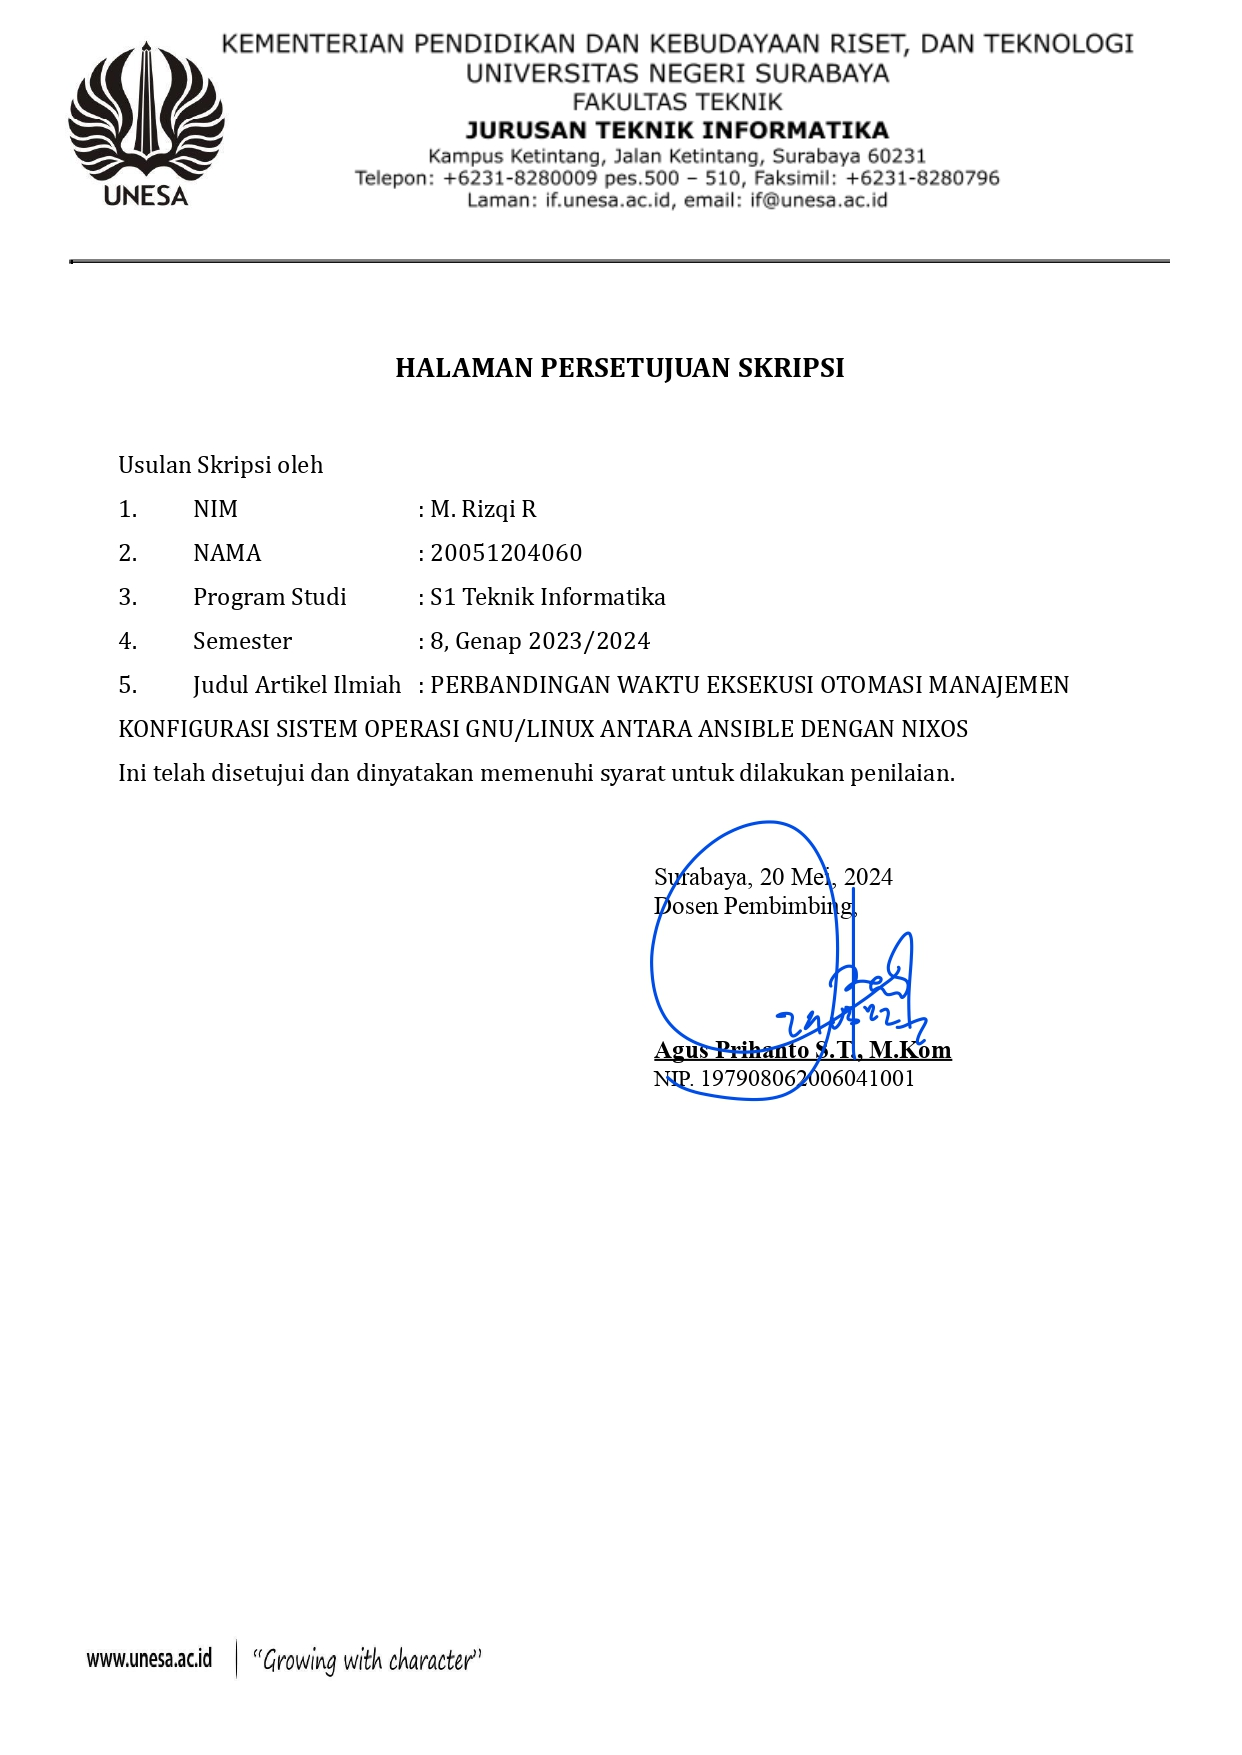
\includegraphics[scale=0.5]{images/Halaman Persetujuan Penilaian.jpg};
	\end{centering}
\end{figure}
\clearpage
% \chapter*{HALAMAN PERSETUJUAN SKRIPSI}
% \begin{adjustwidth}{0.0cm}{}
% 	\begin{tabular}{@{}lcp{0.6\linewidth}}
% 		Nama Mahasiswa & : & M. Rizqi R                                    \\
% 		NIM            & : & 20051204034                                   \\
% 		Judul          & : & PERBANDINGAN WAKTU EKSEKUSI OTOMASI MANAJEMEN
% 		KONFIGURASI SISTEM OPERASI GNU/LINUX ANTARA ANSIBLE DENGAN NIXOS   \\
% 	\end{tabular}
%
% 	\vspace{1cm}
% 	\noindent
% 	Ini telah disetujui dan dinyatakan memenuhi syarat untuk dilakukan penelitian.\\
%
% 	\vspace{5cm}
%
% 	\noindent
% 	Surabaya, 11 Juni 2024\\
% 	Dosen Pembimbing,\\
% 	\vspace{2cm}
%
% 	\noindent
% 	Agus Prihanto, S.T., M.Kom. \\
% 	NIP. 197908062006041001\\
%
% \end{adjustwidth}
\newpage
\chapter*{HALAMAN PENGESAHAN}
\begin{adjustwidth}{0pt}{}
	\begin{tabular}{@{}lcp{0.7\linewidth}}
		Skripsi Oleh & : & M. Rizqi R                                                 \\
		NIM          & : & 20051204034                                                \\
		Judul        & : & \raggedright Perbandingan Waktu Eksekusi Otomasi Manajemen
		Konfigurasi Sistem Operasi GNU/Linux Antara Ansible dengan NixOS              \\
	\end{tabular}

	\noindent Ini telah dipertahankan dihadapan dewan penguji pada tanggal 6 Juni 2024 \\
\end{adjustwidth}
\chapter*{HALAMAN PERSEMBAHAN}
\begin{adjustwidth}{0pt}{}
	Skripsi ini saya tujukan dan perembahkan kepada:
	\begin{enumerate}[nolistsep]
		\item Allah SWT, oleh karena rahmat dan hidayah-Nya, serta segala
		      kenikamatan duniawi sehingga skripsi ini dapat ditulis dan disusun dengan
		      baik dan selesai pada waktunya.
		\item Orang tua terkasih, Bapak Wahyu Diarto dan Ibu Elmi Solichah yang
		      selalu mendukung peneliti dalam segala aspek terutama menempuh
		      pendidikan.
		\item Adik-adik peneliti, yaitu M. Hilman AS dan Anis Wahyu yang secara
		      tidak langsung memberi hiburan kepada peneliti ketika pulang ke rumah.
		\item Teman-teman Asisten Laboratorium Jaringan Komputer dan Asisten
		      Laboratorium Sistem Informasi, terutama Dani Maulana Ferdiansyah, Jerry
		      Yan Krismanto, Firdaus Bagus Wicaksono, serta anggota Aslab lain yang
		      membantu peneliti baik dalam proses penelitian maupun pemberkasan.
		\item Rekan selingkup Teknik Informatika, khususnya Ahmad Fikry Husaini,
		      Dito Arya Saputra, Mochammad Subhan Zuliananta, Richardo Sinulingga yang
		      telah menemani peneliti bermain game saat jenuh.
		\item Vimjoyer dan IogaMaster atas channel YouTube dan forum Discord yang
		      telah membantu dalam mempelajari NixOS
		\item Diri sendiri, yang selalu mencoba untuk bangkit kembali dari
		      kemalasan untuk mengerjakan skripsi sehingga dapat lulus tepat waktu dan
		      tidak membayar UKT untuk penambahan semester.
	\end{enumerate}
\end{adjustwidth}
\newpage
\tableofcontents
\newpage
\listoftables
\newpage
\listoffigures
% bab I

\fancypagestyle{mystyle}{
	\fancyhf{} % Clear all header and footer fields
	\fancyhead[LE]{\thepage} % Odd page numbers on the left
	\fancyhead[RO]{\thepage} % Even page numbers on the right
	\renewcommand{\headrulewidth}{0pt} % Remove the header line
	\renewcommand{\marginparwidth}{0pt}
	% \renewcommand{\marginparsep}{-10pt}
}
\chapter{PENDAHULUAN}
\pagestyle{mystyle}
\pagenumbering{arabic}
\section{Latar Belakang}
\begin{adjustwidth}{0.70cm}{}

	\hspace\parindent
	Pentingnya melakukan manajemen konfigurasi dengan tujuan untuk menghindari
	penulisan manual konfigurasi sistem operasi secara manual setiap kali
	menyiapkan sistem operasi. Manajemen konfigurasi juga digunakan untuk
	mencapai konsistensi dalam setiap kali penerapan sehingga hasil akhir yang
	diinginkan akan sama setiap kali dilakukan.

	Terdapat beberapa \textit{tool} untuk melakukan manajemen konfigurasi sistem operasi,
	terutama untuk sistem operasi berbasis GNU/Linux. Ansible dan NixOS menjadi
	dua dari banyak pilihan untuk melakukan manajemen sistem operasi. Keduanya
	memiliki tujuan memudahkan proses manajemen konfigurasi dan memastikan hasil
	akhir yang diinginkan akan sama setiap kali eksekusi.

	Ansible adalah perangkat lunak otomatisasi TI baris perintah yang ditulis
	dalam bahasa Python. Aplikasi ini dapat mengonfigurasi sistem, menerapkan
	perangkat lunak, dan mengatur alur kerja tingkat lanjut untuk mendukung
	penerapan aplikasi, pembaruan sistem, dan banyak lagi \parencite{AnsibleRedHat}.

	Ansible memungkinkan kita mendeklarasikan konfigurasi sistem operasi kita dalam
	sebuah Ansible Playbook. Ansible Playbook akan dijalankan pada sebuah sistem
	yang telah memiliki sistem operasi. Konfigurasi Ansible Playbook ditulis
	menggunakan format yml yang merupakan format khusus untuk konfigurasi baik
	sistem maupun aplikasi. Ansible akan menjalankan setiap perintah pada sistem
	operasi yang telah di install secara otomatis satu per satu. Ansible
	memungkinkan kita melakukan setup banyak sistem sekaligus dengan konfigurasi
	yang telah ada. Diharapkan dari Ansible adalah sistem-sistem yang terdaftar
	memiliki hasil akhir yang sama.

	NixOS adalah sistem operasi berbasis GNU/Linux yang dibangun dengan Nix build
	system \parencite{hownixworks} . NixOS menggunakan file dalam format “.nix”
	yang disebut sebagai NixOS module untuk mendeklarasikan sebuah sistem. Dalam
	file tersebut terdapat seluruh konfigurasi sistem mulai dari
	\textit{bootloader, packages, users, system services.}

	Apa yang tertulis dalam module tersebut adalah manifestasi dari sistem yang
	dideklarasikan menggunakan bahasa nix yang merupakan bahasa pemrograman
	fungsional. Ini menghasilkan konfigurasi sistem operasi yang \textit{reproducible}
	sehingga dapat digunakan berkali-kali pada waktu yang berbeda dan
	menghasilkan manifestasi yang tetap.

	Banyak kelebihan dan beberapa kekurangan yang dimiliki oleh metode deklaratif
	dari NixOS dan metode campuran (imperatif dan deklaratif) dari Ansible.
	Berdasarkan landasan tersebut, maka penulis ingin meneliti dan membandingkan
	dari segi performa waktu eksekusi yang dibutuhkan oleh masing-masing
	\textit{tool} manajemen konfigurasi dengan hasil akhir konfigurasi yang serupa.
\end{adjustwidth}
\vspace{3mm}
\section{Rumusan Masalah}

\begin{adjustwidth}{0.70cm}{}
	Adapun rumusan masalah berdasarkan latar belakang diatas yaitu:
	\begin{enumerate}[leftmargin=0.45cm, nolistsep]
		\item Bagaimana membuat sistem GNU/Linux yang terdeklarasi menggunakan \textit{tool}
		      manajemen konfigurasi dengan konfigurasi yang serupa.
		\item Berapa lama waktu eksekusi \textit{tool} manajemen konfigurasi yang diimplementasikan.
	\end{enumerate}
\end{adjustwidth}
\section{Tujuan}

\begin{adjustwidth}{0.70cm}{}
	Adapun tujuan dalam penelitian ini adalah:
	\begin{enumerate}[leftmargin=0.45cm, nolistsep]
		\item Membuat sistem GNU/Linux yang terdeklarasi menggunakan NixOS dan
		      Ansible dengan target akhir hasil konfigurasi yang serupa.
		\item Mengukur waktu eksekusi \textit{tool} manajemen konfigurasi NixOS menggunakan nixos-rebuild
		      dan Ubuntu menggunakan Ansible
	\end{enumerate}
\end{adjustwidth}
\vspace{3mm}
\section{Manfaat}

\begin{adjustwidth}{0.70cm}{}
	Manfaat yang dapat dihasilkan dari penelitian ini antara lain:
	\begin{enumerate}[leftmargin=0.45cm, nolistsep]
		\item Efisiensi waktu dalam melakukan manajemen konfigurasi sistem operasi berbasis GNU/Linux.
		\item Konfigurasi sebuah sistem menjadi deklaratif dalam baris kode.
		\item Mengurangi terjadinya human error dalam mengerjakan konfigurasi dan tugas yang berulang-ulang.
		\item Mendapatkan hasil akhir yang konsisten dari penerapan \textit{tool} manajemen konfigurasi.
	\end{enumerate}
\end{adjustwidth}
\vspace{3mm}
\section{Batasan Masalah}

\begin{adjustwidth}{0.70cm}{}
	Adapun batasan masalah yang digunakan untuk menghindari penyimpangan dari judul dan tujuan adalah sebagai berikut:
	\begin{enumerate}[leftmargin=0.45cm, nolistsep]
		\item Tools yang digunakan untuk manajemen konfigurasi adalah Ansible dan
		      NixOS.
		\item Kasus studi dalam menggunakan NixOS menggunakan file konfigurasi
		      dasar, flake, dan home-manager.
		\item Manajemen konfigurasi yang dilakukan meliputi setup dari sistem
		      kosong ke konfigurasi yang diinginkan oleh penulis dimana hasil akhirnya
		      serupa.
		\item Perbandingan akan dilihat berdasarkan waktu yang dibutuhkan untuk
		      eksekusi penerapan konfigurasi.
		\item Untuk nixos-rebuild hanya dijalankan di target NixOS dan Ansible hanya
		      akan dijalankan di Ubuntu menggunakan \textit{apt package manager}.
	\end{enumerate}
\end{adjustwidth}
%bab II
\pagebreak
\hspace{0pt}
\vfill
\begin{center}
	Halaman ini sengaja dikosongkan
\end{center}
\vfill
\pagebreak

\chapter{KAJIAN PUSTAKA}
\section{Penelitian Terdahulu}
\begin{adjustwidth}{0.70cm}{}

	\hspace\parindent
	Sudah ada penelitian terdahulu terkait otomasi menggunakan Ansible. Salah
	satu diantaranya adalah yang dilakukan oleh Thufail Qolba Aufar yang
	berjudul \textit{“Configuration Management dengan Ansible dan Telegram Untuk
		Automasi Laboratorium Komputer di JTIK”} pada tahun 2023 \parencite{thufail23}. Dalam penelitia
	tersebut menggunakan Ansible sebagai \textit{tool} manajemen konfigurasi
	laboratorium komputer. Sistem operasi yang digunakan oleh target host
	adalah Windows dan Ansible Module yang digunakan adalah win\_chocolatey yang
	merupakan modul untuk chocolatey \textit{package manager} di Windows.

	Sistem Configuration Management dengan Ansible dan Telegram berhasil dibuat
	sesuai dengan fungsionalitas dan rancangan yang telah dibuat. Hal Ini
	dibuktikan dari pengujian fungsionalitas dengan black box testing yang telah
	dilakukan bahwa setiap tugas dieksekusi dapat berjalan dengan persentase
	keberhasilan sebesar 100\%.

	Penelitian untuk otomasi dan manajemen konfigurasi distribusi GNU/Linux
	ditulis oleh Putu Hariyadi dan Khairan Marzuki dengan judul \textit{“Implementation
		Of Configuration Management Virtual Private Server Using Ansible”} pada
	tahun 2020 \parencite{hariyadi2020}. Pada penelitian tersebut, Ansible digunakan untuk melakukan
	otomasi pembuatan container pada PVE (Proxmox Virtual Environment) yang
	bertujuan untuk menyiapkan lingkungan \textit{high availability} sebagai media
	praktikum kelompok untuk dosen, mahasiswa, dan asisten laboratorium.

	Hasilnya adalah manajemen otomasi VPS secara keseluruhan bekerja dengan baik
	dan dapat diterapkan di Proxmox Virtual Environment (PVE) cluster. Playbook
	dapat memulai dan menghentikan containers per kelompok siswa secara dinamis
	berdasarkan jadwal praktikum.

	Penelitian terkait penggunaan NixOS sebagai manajemen konfigurasi telah
	dijabarkan oleh Kalle Kumpulainen dalam tesis ber judul \textit{“NixOS:
		Järjestelmäkonfiguraation Hallintaan Erikoistunut Linux-jakelu”} pada tahun
	2019. Dalam tesis tersebut dituliskan bagaimana NixOS menjadi sebuah
	distribusi GNU/Linux yang hampir keseluruhan sistemnya terdeklarasi dalam
	bentuk konfigurasi.Terkait apa saja perbedaan dibandingkan dengan
	distribusi GNU/Linux yang telah ada \parencite{kumpulainen_2019_nixos}.

	Ansible juga pernah diteliti dan dibandingkan dengan metode manajemen
	konfigurasi konvensional yaitu shell scripting dengan BASH. Penelitian ini
	dilakukan oleh Tedi Alfiandi, T.M Diansyah, dan Risko Liza yang tertuang
	dalam “Analisis Perbandingan Manajemen Konfigurasi Menggunakan Ansible dan
	Shell Script Pada \textit{Cloud Server Deployment} AWS” pada tahun 2020. Didapat
	kesimpulan bahwa penggunaan tool manajemen konfigurasi dapat memperingkas
	pekerjaan dalam membangun \textit{web server} \parencite{alfiandi_2020_analisis}.

	Dalam penelitian lain yang dilakukan oleh Muh. Akromi Arya Pratama dan I Putu
	Hariyadi, dalam sebuah jurnal berjudul “Otomasi Manajemen dan Pengawasan
	Linux Container (LXC) Pada Proxmox VE Menggunakan Ansible”. Ansible digunakan
	untuk mempermudah proses otomasi pembuatan LXC pada proxmox untuk praktikum
	SMKN 6 Mataram. Kesimpulan yang didapat ialah Ansible mampu melakukan otomasi
	untuk membuat, menjalankan, menghentikan dan menghapus LXC serta mengatur
	\textit{user permission} dalam lingkup \textit{batch} \parencite{pratama_2021_otomasi}.\\
\end{adjustwidth}

\begin{longtable}[H]{|c|p{0.22\textwidth}|p{0.15\textwidth}|R|}
	\caption{Penelitian Terdahulu} \tabularnewline  \hline
	\centering\raisebox{-0.2cm}{\centering\textbf{No.}} & \centering\raisebox{-0.2cm}{{\textbf{Judul}}}                                                                                                                   & \centering{\textbf{Nama Peneliti}}       & \centering\raisebox{-0.2cm}{\centering{\textbf{Kesimpulan}}} \\
	\endfirsthead
	\hline
	\centering\raisebox{-0.2cm}{\centering\textbf{No.}} & \centering\raisebox{-0.2cm}{{\textbf{Judul}}}                                                                                                                   & \centering{\textbf{Nama Peneliti}}       & \centering\raisebox{-0.2cm}{\centering{\textbf{Kesimpulan}}} \\
	\endhead
	\hline
	1                                                   & \textit{Configuration Management} dengan Ansible dan Telegram Untuk
	Automasi Laboratorium Komputer di JTIK              & Thufail Qolba Aufar                                                                                                                                             & Sistem
	Configuration Management dengan Ansible dan Telegram berhasil dibuat sesuai
	dengan fungsionalitas dan rancangan yang telah dibuat. Hal Ini dibuktikan
	dari pengujian fungsionalitas dengan black box testing yang telah dilakukan
	bahwa setiap tugas dieksekusi dapat berjalan dengan persentase keberhasilan
	sebesar 100.                                                                                                                                                                                                                                                                                                                    \\
	\hline
	2                                                   & \textit{Implementation Of Configuration Management Virtual Private Server
	Using Ansible}                                      & Putu Hariyadi, Khairan Marzuki                                                                                                                                  & Manajemen otomasi VPS
	secara keseluruhan bekerja dengan baik dan dapat diterapkan di Proxmox
	Virtual Environment (PVE) cluster. Playbook dapat memulai dan menghentikan
	containers per kelompok siswa secara dinamis berdasarkan jadwal praktikum.                                                                                                                                                                                                                                                      \\

	\hline
	3                                                   & \textit{NixOS: Järjestelmä konfiguraation Hallintaan Erikoistunut Linux
	jakelu}                                             & Kalle Kumpulai nen                                                                                                                                              & Distribusi ini pada awalnya dibuat untuk
	memecahkan masalah asli distribusi perangkat lunak dan manajemen konfigurasi
	sistem operasi,                                                                                                                                                                                                                                                                                                                 \\ \hline &  &  & seperti keamanan dan determinisme fungsi yang diinginkan.
	Untuk mengatasi masalah ini, NixOS diimplementasikan sejak awal dengan cara
	yang sangat tidak biasa dibandingkan dengan distribusi Linux terkenal
	lainnya.                                                                                                                                                                                                                                                                                                                        \\

	\hline
	4                                                   & Analisis Perbandingan Manajemen Konfigurasi Menggunakan Ansible dan Shell
	Script Pada Cloud Server Deployment AWS             & Tedi Alfiandi, T.M Diansyah, Risko
	Liza                                                & Penggunaan tool manajemen konfigurasi dapat memperingkas pekerjaan
	dalam membangun web server                                                                                                                                                                                                                                                                                                      \\
	\hline

	5                                                   & Otomasi Manajemen dan Pengawasan Linux Container (LXC) Pada Proxmox VE Menggunakan Ansible
	                                                    & Muh. Akromi Arya Pratama dan I Putu Hariyadi
	                                                    & Ansible mampu melakukan otomasi untuk membuat, menjalankan, menghentikan dan menghapus LXC serta mengatur \textit{user permission} dalam lingkup \textit{batch}                                                                                                           \\
	\hline
\end{longtable}

\section{Manajemen Konfigurasi}
\begin{adjustwidth}{20pt}{}

	Manajemen konfigurasi adalah metode dimana sebuah sistem di manajemen
	menggunakan file-file yang mendeskripsikan apa yang harus dilakukan sistem
	tersebut. Harapan dari hasil file-file konfigurasi ini adalah konsistensi
	pada hasil akhir setelah konfigurasi tersebut dijalankan. Metode ini juga
	bertujuan untuk meningkatkan efisiensi dalam replikasi dan manajemen sistem
	sehingga administrator tidak melakukan konfigurasi dari nol hingga selesai
	secara berulang.
\end{adjustwidth}
\section{Imperatif}
\begin{adjustwidth}{20pt}{}

	Dalam konteks manajemen konfigurasi, imperatif merupakan metode dimana
	administrator menetapkan langkah-langkah yang perlu dilakukan sebuah sistem
	untuk mencapai keadaan tertentu. Dalam kasus penelitian ini adalah Ansible
	dimana setiap definisi yang kita tulis dalam Ansible Playbook akan dijalankan
	satu persatu dari awal hingga akhir dengan harapan bahwa apa yang kita
	definisikan dalam Playbook tercapai.
\end{adjustwidth}
\section{Deklaratif}
\begin{adjustwidth}{20pt}{}

	Dalam konteks manajemen konfigurasi, deklaratif merupakan metode dimana
	administrator menetapkan rincian tentang keadaan akhir sistem dalam file-file
	konfigurasi. Dalam kasus penelitian ini adalah NixOS Module yang berisikan
	rincian hasil akhir yang kita inginkan dalam NixOS. NixOS Module akan di
	evaluasi oleh Nix build system untuk menggapai tujuan ini.
\end{adjustwidth}
\section{Immutable Distro}
\begin{adjustwidth}{20pt}{}

	Immutable Distro adalah kategori distribusi GNU/Linux yang dimana sistem
	operasi read-only yang tidak mengijinkan modifikasi di root file system. Ini
	berarti kita tidak bisa dengan mudah memodifikasi OS. Ini termasuk file
	sistem, berkas, aplikasi, bahkan konfigurasi. Bahkan sebagai administrator,
	kita tidak bisa memodifikasi distribusi tersebut.
\end{adjustwidth}
\section{Reproducible}
\begin{adjustwidth}{20pt}{}

	Dalam konteks manajemen konfigurasi, reproducible merujuk pada hasil akhir
	yang konsisten setiap kali konfigurasi diterapkan.
\end{adjustwidth}
\section{Repeatable}
\begin{adjustwidth}{20pt}{}

	Dalam konteks manajemen konfigurasi, repeatable merujuk pada tahapan-tahapan
	yang dapat diulang dengan tujuan hasil serupa.
\end{adjustwidth}
\section{NixOS}
\begin{adjustwidth}{20pt}{}

	Distribusi sistem operasi GNU/Linux yang terintegrasi dengan Nix package
	manager dimana konfigurasi sistem operasi dideklarasikan dalam Nix Module.
\end{adjustwidth}
\section{Ansible}
\begin{adjustwidth}{20pt}{}

	Ansible adalah perangkat lunak otomatisasi TI baris perintah yang ditulis dalam
	bahasa Python. Aplikasi ini dapat mengonfigurasi sistem, menerapkan perangkat
	lunak, dan mengatur alur kerja tingkat lanjut untuk mendukung penerapan
	aplikasi, pembaruan sistem, dan banyak lagi (RedHat, 2022a)
\end{adjustwidth}
\section{YAML}
\begin{adjustwidth}{20pt}{}

	Bahasa serialisasi data yang bisa dibaca oleh manusia. YAML umumnya digunakan
	untuk file konfigurasi dan aplikasi dimana data disimpan atau
	ditransmisikan.(Wikipedia)
\end{adjustwidth}
\section{BASH}
\begin{adjustwidth}{20pt}{}

	Bourne-Again Shell (BASH) adalah Unix-shell dan bahasa perintah yang biasanya
	berjalan di jendela text dimana pengguna mengetik perintah yang mengakibatkan
	aksi
\end{adjustwidth}
\section{NixOS Module}
\begin{adjustwidth}{20pt}{}

	Module yang berisi Nix expression dengan struktur yang spesifik dan digunakan
	untuk membangun konfigurasi Nix yang utuh.
\end{adjustwidth}
\section{Flake}
\begin{adjustwidth}{20pt}{}
	Nix flakes menyediakan cara standar untuk menulis ekspresi Nix (dan juga paket-paket) yang ketergantungannya disematkan dalam file kunci, sehingga meningkatkan kemampuan reproduksi instalasi Nix.
\end{adjustwidth}
\section{Home Manager}
\begin{adjustwidth}{20pt}{}

	Home Manager adalah sistem untuk mengelola lingkungan pengguna dengan
	menggunakan manajer paket Nix. Dengan kata lain, Home Manager memungkinkan
	Anda menginstall perangkat lunak secara deklaratif pada profil user Anda,
	daripada menggunakan nix-env,mengelola dotfile di direktori home pengguna
	Anda.
\end{adjustwidth}
\section{Virtualisasi}
\begin{adjustwidth}{20pt}{}

	Virtualisasi merupakan proses berbasis perangkat lunak yang membagi komputer
	tunggal menjadi beberapa mesin virtual / virtual machine, tiap-tiap mesin
	virtual memiliki sistem operasi dan aplikasi miliknya sendiri (IBM, 2024)
\end{adjustwidth}
% bab III
\chapter{METODE PENELITIAN}
Metodologi yang digunakan untuk penelitian ini memiliki beberapa tahapan
sebagai pedoman agar hasil yang dicapai sesuai dan tidak menyimpang dari tujuan
yang telah ditentukan sebelumnya.

\section{Metode Penelitian}
\begin{adjustwidth}{20pt}{}

	\hspace\parindent
	Metode yang diterapkan pada penelitian ini adalah metode experimental design.
	Penerapan metode bertujuan untuk menganalisa perbandingan manajemen
	konfigurasi sistem operasi GNU/Linux antara Ansible dengan NixOS.
	% \vspace{-20pt}

	\begin{figure}[h]
		\centering
		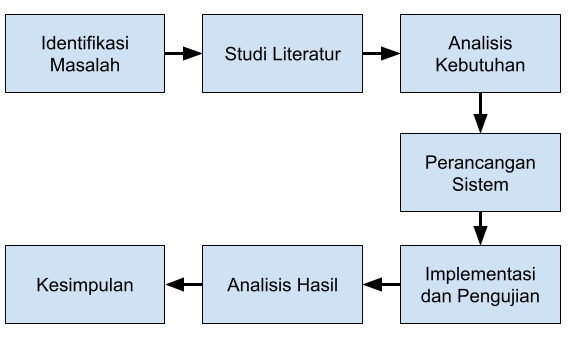
\includegraphics[width=0.8\textwidth]{images/metpen.png}
		\caption{Daigram \textit{experimental design}}
	\end{figure}

\end{adjustwidth}
\begin{adjustwidth}{20pt}{}
	\hspace\parindent
	Berikut merupakan alur tahapan yang dilakukan dalam penelitian ini.
	Pada gambar 3.1, dapat diketahui tahapan penelitian yang akan diterapkan
	pada penelitian ini, yaitu:
\end{adjustwidth}
\begin{adjustwidth}{20pt}{}
	\subsection{Identifikasi Masalah}
	\begin{adjustwidth}{20pt}{}
		Tahapan awal untuk melakukan penelitian merupakan identifikasi masalah. Pada
		tahapan ini, permasalahan yang diidentifikasi mengenai manajemen konfigurasi
		di GNU/Linux untuk mempersingkat waktu konfigurasi dan membuat sistem yang
		terdeklarasi. Peneliti akan membuat konfigurasi sistem operasi GNU/Linux
		menggunakan Ansible dan NixOS dengan kebutuhan yang sama dengan tujuan untuk
		membandingkan efisiensi kecepatan penerapan \textit{tool} manajemen konfigurasi.
	\end{adjustwidth}
\end{adjustwidth}
\begin{adjustwidth}{20pt}{}
	\subsection{Studi Literatur}
	\begin{adjustwidth}{20pt}{}
		Peneliti mencari literatur yang relevan untuk menjadi referensi pendukung dalam
		penelitian. Literatur yang digunakan dalam penelitian ini berhubungan
		dengan penerapan manajemen konfigurasi yang didapat dari berbagai macam
		sumber seperti buku, artikel, jurnal nasional maupun internasional.
	\end{adjustwidth}
\end{adjustwidth}
\begin{adjustwidth}{20pt}{}
	\subsection{Analisis Kebutuhan}
	\begin{adjustwidth}{20pt}{}
		Tahap ini bertujuan untuk mendapatkan pemahaman yang menyeluruh dan terperinci
		tentang kebutuhan utama sistem seperti yang didefinisikan agar tujuan
		tercapai, yang kemudian secara jelas didefinisikan, ditinjau dan disepakati
		bersama.
	\end{adjustwidth}
\end{adjustwidth}
\begin{adjustwidth}{20pt}{}
	\subsection{Perancangan Sistem}
	\begin{adjustwidth}{20pt}{}
		Perancangan dilakukan dengan menerapkan manajemen konfigurasi pada mesin
		virtual agar mendapatkan hasil waktu yang dibutuhkan untuk menerapkan
		konfigurasi. Berikut flowchart proses dari penerapan konfigurasi yang akan
		dibuat:
		\begin{figure}[!htb]
			\centering
			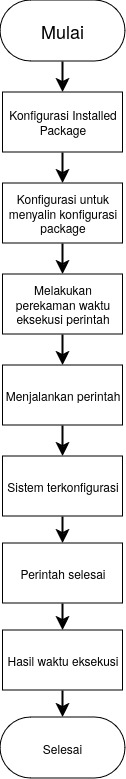
\includegraphics[width=0.2\textwidth]{images/flow.jpg}
			\caption{\textit{flowchart} manajemen konfigurasi}
		\end{figure}
	\end{adjustwidth}
\end{adjustwidth}
\newpage
\begin{adjustwidth}{20pt}{}
	\subsection{Implementasi dan Pengujian}
	\begin{adjustwidth}{20pt}{}
		Pada tahap ini, rancangan konfigurasi yang sudah dibuat akan
		diimplementasikan sesuai alur kerja konfigurasi yang telah dibuat pada
		lingkungan mesin virtual agar lebih efisien dan lebih terisolasi. Instalasi
		dan konfigurasi dilakukan sesuai referensi dokumentasi dari masing-masing
		\textit{tool} manajemen konfigurasi. Kustomisasi dari perangkat lunak yang
		diperlukan tergantung pada kebutuhan penelitian. Parameter pengujian yang
		akan dilakukan adalah menguji kecepatan waktu eksekusi dan \textit{reproducibility} dari
		masing-masing \textit{tool} manajemen konfigurasi.
	\end{adjustwidth}
\end{adjustwidth}
\begin{adjustwidth}{20pt}{}
	\subsection{Analisis Hasil}

	\begin{adjustwidth}{20pt}{}
		Pada tahap ini, hasil dari implementasi dan pengujian akan dianalisis untuk
		mengetahui kecepatan penerapan konfigurasi dan konsistensi \textit{tool} manajemen
		konfigurasi.Untuk mengetahui waktu yang dibutuhkan oleh \textit{tool} manajemen
		konfigurasi untuk menerapkan konfigurasi, akan digunakan perintah “time”.
		Untuk mengetahui konsistensi penerapan, akan dilihat dari hasil akhir konfigurasi
		setelah diterapkan secara berulang.
	\end{adjustwidth}
\end{adjustwidth}

\begin{adjustwidth}{20pt}{}
	\subsection{Kesimpulan}

	\begin{adjustwidth}{20pt}{}
		Tahapan terakhir dalam penelitian ini akan dilakukan penarikan kesimpulan
		dan pemberian saran dari seluruh penelitian yang telah dilakukan
		berdasarkan rumusan masalah yang telah dijelaskan sebelumnya. Hasil dari
		pengujian \textit{tool} manajemen konfigurasi dapat menjadi jawaban dari masalah
		yang telah dijelaskan, serta data dari penelitian diharapkan berguna dalam
		efisiensi dan konsistensi penerapan manajemen konfigurasi sistem operasi
		GNU/Linux dan dapat menjadi referensi penelitian berikutnya.
	\end{adjustwidth}
\end{adjustwidth}
\vspace{3mm}
\section{Analisis Kebutuhan}

\begin{adjustwidth}{20pt}{}
	Analisis kebutuhan merupakan analisis yang dibutuhkan untuk menentukan detail
	kebutuhan pada penelitian analisis perbandingan manajemen konfigurasi sistem
	operasi GNU/Linux antara Ansible dengan NixOS. Penelitian ini mengotomasi
	konfigurasi sistem operasi GNU/Linux dan membuat sistem menjadi terdeklarasi.
	Sehingga dibutuhkan perangkat-perangkat yang dapat mendukung agar penelitian
	ini berjalan sesuai tujuan. Berikut merupakan kebutuhan yang dibagi menjadi
	beberapa bagian, yaitu:
\end{adjustwidth}
\begin{adjustwidth}{20pt}{}
	\subsection{Kebutuhan perangkat keras (\textit{hardware})}
	\begin{adjustwidth}{20pt}{}
		Perangkat keras yang diperlukan guna tujuan penelitian yaitu Laptop sebagai
		uji coba dengan spesifikasi berikut:
	\end{adjustwidth}
	\begin{adjustwidth}{5mm}{}
		\begin{tabular}{ll}
			Processor      & : Intel Core i5 11400H         \\
			RAM            & : 24 GB                        \\
			SSD            & : 1 TB                         \\
			Sistem Operasi & : NixOS 24.05 (Uakari) x86\_64 \\
		\end{tabular}
	\end{adjustwidth}
	\subsection{Kebutuhan perangkat lunak (\textit{software}) }
	\vspace{-2mm}
	\begin{adjustwidth}{20pt}{}
		Perangkat lunak berfungsi untuk pengoperasian sistem pada penelitian ini.
		Pada penelitian ini, sistem operasi yang digunakan berbasis GNU/Linux.
		\begin{longtable}[H]{|c|p{2.5cm}|>{\raggedright\arraybackslash}p{5.5cm}|}
			\caption{Kebutuhan perangkat lunak} \tabularnewline
			\hline
			\centering\raisebox{-0.4cm}{\textbf{No.}} & \centering\textbf{Nama Perangkat Lunak} & \centering\raisebox{-0.4cm}{\textbf{Keterangan}}                          \\
			\endfirsthead
			\hline
			\centering\raisebox{-0.4cm}{\textbf{No.}} & \centering\textbf{Nama Perangkat Lunak} & \centering\raisebox{-0.4cm}{\textbf{Keterangan}}                          \\
			\endhead
			\hline
			1                                         & Ansible                                 & Alat yang digunakan untuk manajemen konfigurasi                           \\
			\hline
			2                                         & NixOS                                   & Sistem Operasi dengan fitur manajemen konfigurasi                         \\
			\hline
			3                                         & Ubuntu Server 24.04 LTS                 & Sistem Operasi yang digunakan untuk target Ansible                        \\
			\hline
			4                                         & Nix Flakes                              & Alat yang digunakan untuk manajemen \textit{inputs} pada NixOS            \\
			\hline
			5                                         & Home Manager                            & Alat yang digunakan untuk manajemen konfigurasi level pengguna pada NixOS \\
			\hline
			6                                         & \textit{time}                           & Alat yang digunakan untuk mencatat lama waktu eksekusi perintah           \\
			\hline
		\end{longtable}
	\end{adjustwidth}
\end{adjustwidth}

\section{Perancangan Sistem}

\begin{adjustwidth}{20pt}{}
	Perancangan sistem dilakukan untuk membuat desain perencanaan arsitektur
	sistem yang akan dibangun dapat berjalan sesuai dengan tujuan penelitian.
	\subsection{Perancangan Virtual Machine}
	\begin{adjustwidth}{20pt}{}
		Perancangan sistem pada penelitian ini secara keseluruhan menggunakan enam
		\textit{virtual machine}, yang terdiri dari tiga \textit{instance} Ubuntu
		Server 24.04 LTS dan tiga \textit{instance} NixOS minimal.
		Satu dari tiga \textit{virtual machine} bersifat sebagai \textit{master}
		dan dua sebagai \textit{target}.
		\begin{table}[H]
			\centering
			\caption{Spesifikasi Instance}
			\begin{tabular}{|l|l|}
				\hline
				\multicolumn{2}{|c|}{\textit{Instance} Ansible}    \\
				\hline
				Sistem Operasi           & Ubuntu Server 24.04 LTS \\
				\hline
				Processor                & 2                       \\
				\hline
				Memory                   & 4 GB                    \\
				\hline
				Storage                  & 50 GB                   \\
				\hline
				Jumlah \textit{instance} & 3                       \\
				\hline
				\multicolumn{2}{|c|}{\textit{Instance} NixOS}      \\
				\hline
				Sistem Operasi           & NixOS 23.11             \\
				\hline
				Processor                & 2                       \\
				\hline
				Memory                   & 4 GB                    \\
				\hline
				Storage                  & 50 GB                   \\
				\hline
				Jumlah \textit{instance} & 3                       \\
				\hline
			\end{tabular}
		\end{table}
		Alasan perbedaan target dari Ansible dan NixOS adalah karena nixos-rebuild
		tidak bisa dijalankan pada sistem operasi selain NixOS. Ansible juga tidak
		dapat digunakan di NixOS karena sifat NixOS sendiri yang \textit{immutable}
		membuat metode imperatif untuk konfigurasi sistem operasi tidak memungkinkan.
		Alasan berikutnya adalah dikarenakan kenyataan dilapangan dimana Ubuntu Server
		akan dikonfigurasi menggunakan Ansible dan menggunakan \textit{package manager} apt,
		sedangkan untuk NixOS pasti akan dikonfigurasi menggunakan file konfigurasi ".nix".
	\end{adjustwidth}
	\subsection{Perancangan Topologi}
	\begin{adjustwidth}{20pt}{}
		\hspace\parindent
		Perancangan topologi untuk penelitian ini adalah dengan sistem master dan
		target. Sistem ini akan membuat satu perangkat sebagai pusat kendali dari
		beberapa target yang menjadi endpoint dari manajemen konfigurasi.\\
		\begin{figure}[H]
			\centering
			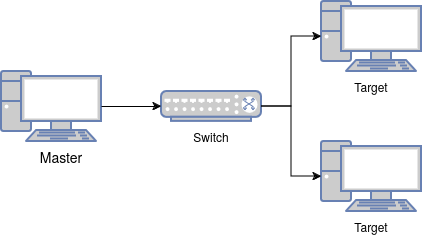
\includegraphics[width=0.8\textwidth]{images/base-topology.png}
			\captionof{figure}{Topologi Pengujian}
		\end{figure}
		Dengan topologi ini, diharapkan penerapan manajemen konfigurasi terpusat
		dan dapat diterapkan di dua mesin target dan memiliki hasil akhir yang sama
		dan konsisten antar mesin.
	\end{adjustwidth}
\end{adjustwidth}
\section{Perancangan Pengujian}

\begin{adjustwidth}{20pt}{}
	\hspace\parindent
	Perancangan pengujian pada penelitian ini akan melakukan instalasi berbagai
	macam perangkat lunak. Perangkat lunak yang diinstall adalah tmux, vim,
	htop. Kemudian akan dilakukan beberapa konfigurasi perangkat lunak
	yaitu konfigurasi untuk tmux, vim, openssh, firewall.

	Kemudian akan dihadirkan service tambahan yaitu berupa \textit{web server}
	menggunakan Nginx. Nginx juga akan dikonfigurasi untuk menampilkan
	\textit{website} sederhana yang kode sumbernya diambil dari
	\textit{repository} Github.
	\begin{figure}[H]
		\centering
		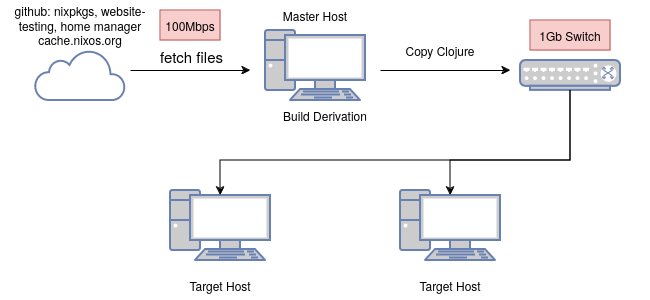
\includegraphics[width=\textwidth]{images/nixos-topology-revision.png}
		\caption{Alur Penerapan Konfigurasi NixOS}
	\end{figure}

	Pada gambar 3.4 merupakan alur penerapan konfigurasi menggunakan NixOS.
	Master akan melakukan \textit{clone} dari \textit{repository} nixpkgs,
	home-manager dan website-testing untuk mengambil konfigurasi sistem serta
	file \textit{website} yang akan di \textit{deploy}. Kemudian \textit{master}
	akan melakukan build untuk konfigurasi keseluruhan sistem sehingga
	menghasilkan nix derivation yang membentuk NixOS. Hasil dari derivation
	tersebut kemudian akan di \textit{copy} dan diterapkan ke dua mesin target.
	\newpage
	\begin{figure}[H]
		\centering
		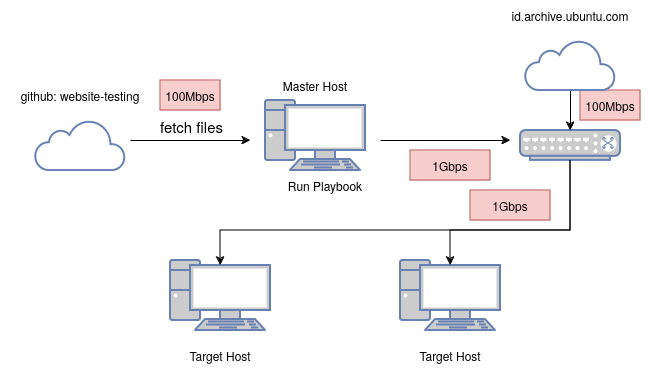
\includegraphics[width=\textwidth]{images/ansible-topology-revision.png}
		\caption{Alur Penerapan Konfigurasi Ansible}
	\end{figure}
	Pada gambar 3.5 merupakan alur penerapan konfigurasi menggunakan Ansible.
	\textit{Master} akan melakukan \textit{clone} dari \textit{repository} github
	website-testing. Kemudian \textit{master} akan mulai menerapkan konfigurasi
	untuk target dan menginstall semua paket yang di definisikan dan melakukan
	konfigurasi yang diinginkan. Masing-masing target dengan sistem operasi
	Ubuntu Server akan mengunduh paket dari \textit{repository}
	id.archive.ubuntu.com.
	Setelah konfigurasi sistem selesai diterapkan kemudian Ansible akan menyalin
	file \textit{website} yang ada di master ke target.

	Setiap kali perintah untuk melakukan konfigurasi di eksekusi, waktu eksekusi
	akan dicatat menggunakan perintah “time”. Eksekusi akan dilakukan secara
	berulang untuk mendapatkan rata-rata waktu yang dibutuhkan untuk menerapkan
	konfigurasi.
	Patut di ingat bahwa \textit{bandwidth} maksimal untuk menuju internet
	adalah 100Mbps dan bandwidth \textit{local connection} adalah 1Gbps.
\end{adjustwidth}
% Time Schedule dihapus saat semhas
% \section{Time Schedule}
% \begin{adjustwidth}{20pt}{}
% 	Berikut \textit{time schedule} yang penulis susun sebagai acuan pelaksanaan
% 	kegiatan:
% 	\begin{table}[H]
% 		\caption{Time Schedule}
% 		\begin{tabular}{|p{2cm}|c|c|c|c|c|c|}
% 			\hline
% 			\multicolumn{1}{|c|}{\multirow{2}{*}{\centering{\textbf{Kegiatan}}}} & \textbf{2023}     & \multicolumn{5}{|c|}{\textbf{2024}}                                                                                 \\
% 			\cline{2-7}
% 			                                                                     & Des               & Jan                                 & Feb               & Mar               & Apr               & Mei               \\
% 			\hline
% 			Identifikasi Masalah                                                 & \cellcolor{green} &                                     &                   &                   &                   &                   \\
% 			\hline
% 			Studi Literatur                                                      &                   & \cellcolor{green}                   &                   &                   &                   &                   \\
% 			\hline
% 			Analisis Kebutuhan                                                   &                   & \cellcolor{green}                   &                   &                   &                   &                   \\
% 			\hline
% 			Perancangan Sistem                                                   &                   &                                     & \cellcolor{green} & \cellcolor{green} &                   &                   \\
% 			\hline
% 			Implementasi dan Pengujian                                           &                   &                                     &                   &                   & \cellcolor{green} &                   \\
% 			\hline
% 			Analisis Hasil                                                       &                   &                                     &                   &                   &                   & \cellcolor{green} \\
% 			\hline
% 			Kesimpulan                                                           &                   &                                     &                   &                   &                   & \cellcolor{green} \\
% 			\hline
% 		\end{tabular}
% 	\end{table}
%
% \end{adjustwidth}
% bab IV
\pagebreak
\hspace{0pt}
\vfill
\begin{center}
	Halaman ini sengaja dikosongkan
\end{center}
\vfill
\pagebreak
\chapter{HASIL PENELITIAN DAN PEMBAHASAN}
Hasil dari penelitian peneliti berupa data-data terkait waktu eksekusi yang
dibutuhkan untuk penerapan manajemen konfigurasi dari eksekusi nixos-rebuild
dan ansible-playbook. Peneliti membangun dua jenis konfigurasi, yaitu
konfigurasi untuk NixOS dan Ansible. Untuk konfigurasi NixOS menggunakan flake
untuk mencapai \textit{reproducibility} dan Home-Manager untuk mengkonfigurasi
aplikasi pengguna.

Untuk konfigurasi Ansible dibuat semirip mungkin dengan konfigurasi NixOS.
Perbedaan nya adalah metode file konfigurasi pada Ansible menggunakan
ansible.posix.synchronize dan ansible.builtin.copy untuk menyalin /
mensinkronisasi file konfigurasi setiap aplikasi dan \textit{services}.
\vspace{3mm}
\section{Implementasi}

\begin{adjustwidth}{20pt}{}
	\subsection{Persiapan Lingkungan NixOS}
	\begin{adjustwidth}{20pt}{}
		Untuk persiapan lingkungan NixOS baik \textit{master} maupun target
		adalah sebagai berikut:
	\end{adjustwidth}
	\subsubsection{Download ISO dan konfigurasi VM}
	\begin{adjustwidth}{20pt}{}
		\textit{Download} ISO NixOS GNOME di \url{https://nixos.org}, kemudian
		install dalam VM Proxmox dengan BIOS (OVMF) UEFI q35 dan CPU Type : host
		agar kita dapat memanfaatkan semua instruction set dari CPU. Lanjutkan
		dengan spesifikasi CPU, RAM, dan HDD seperti yang telah dicantumkan pada
		BAB III. Untuk NixOS pada saat penulisan yaitu versi ISO 23.11 belum
		mendukung \textit{secure boot} secara bawaan. Maka dari itu, perlu untuk
		menonaktifkan \textit{secure boot} pada VM Proxmox agar ISO bisa dipakai.
		Saat booting, \textit{spam} tombol 'Esc' untuk masuk ke \textit{firmware setting} dan
		matikan \textit{Secure Boot} pada bagian \textit{Device Manager
			-\textgreater Secure Boot Configuration -\textgreater Disable secure boot
			next -\textgreater Attempt Secure Boot} kemudian klik spasi dan tekan 'y'.
		Tekan 'F10' untuk menyimpan konfigurasi. Tekan 'Esc' dua kali untuk keluar
		dan pilih 'Reset'. Setelah itu, kita akan disambut dengan GNOME
		\textit{Desktop Environment} seperti berikut:
		\begin{center}
			\begin{figure}[h]
				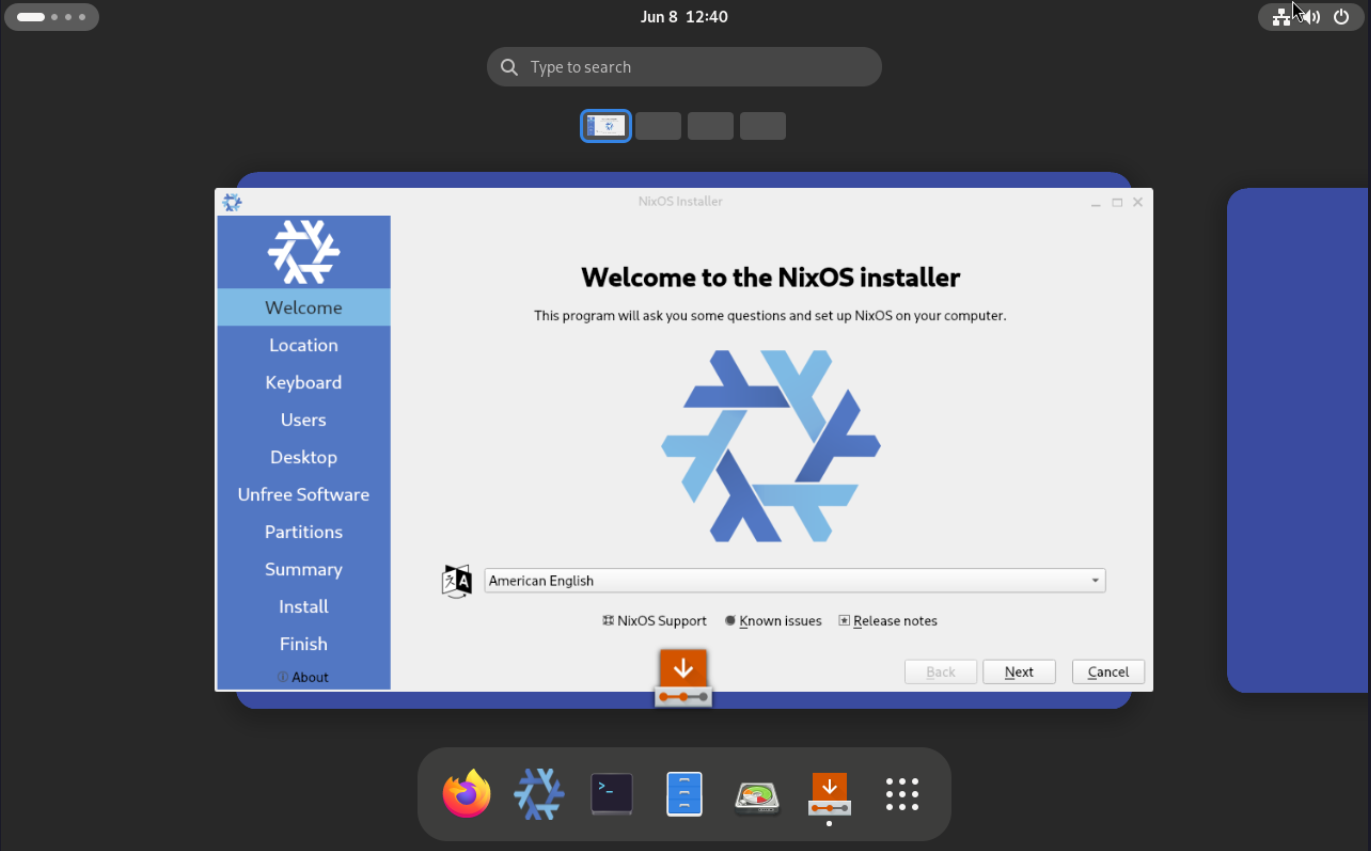
\includegraphics[width=0.95\textwidth]{images/nixos-23.11-installer.png}
				\caption{NixOS 23.11 installer GNOME}
			\end{figure}
		\end{center}
	\end{adjustwidth}

	\subsubsection{Instalasi}
	\begin{adjustwidth}{20pt}{}
		Kemudian kita masuk ke tahap instalasi NixOS sebagai berikut:
		\begin{enumerate}[nolistsep]
			\item Atur lokasi ke Asia/Jakarta.
			      \newpage
			      \begin{figure}[H]
				      \begin{center}
					      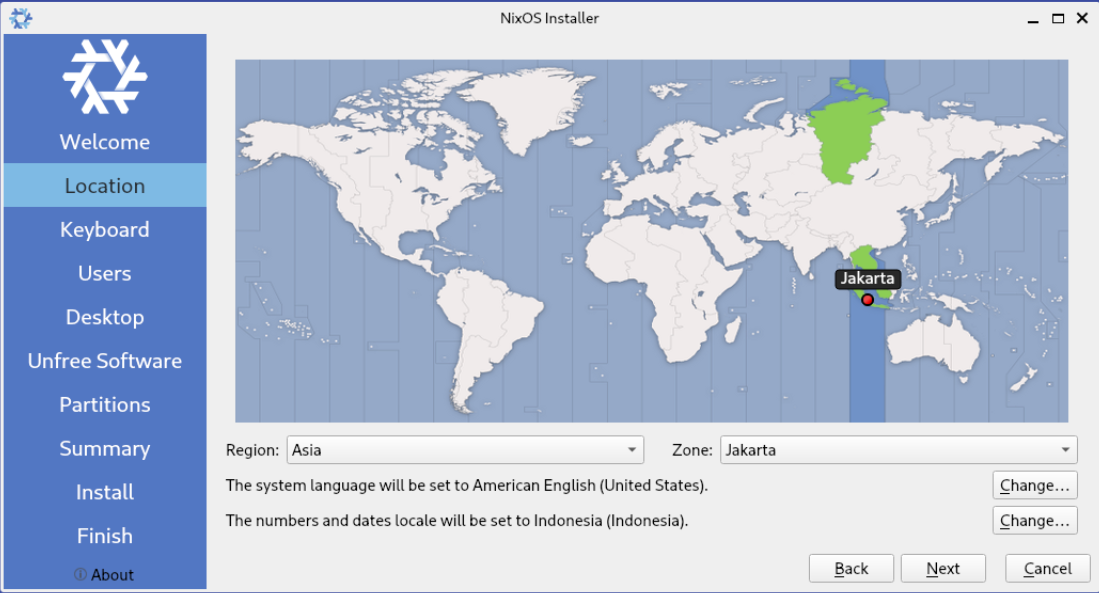
\includegraphics[width=0.95\textwidth]{images/nixos-23.11-location.png}
				      \end{center}
				      \caption{NixOS 23.11 Location}
			      \end{figure}
			\item Atur keyboard ke US default.
			      \begin{figure}[H]
				      \begin{center}
					      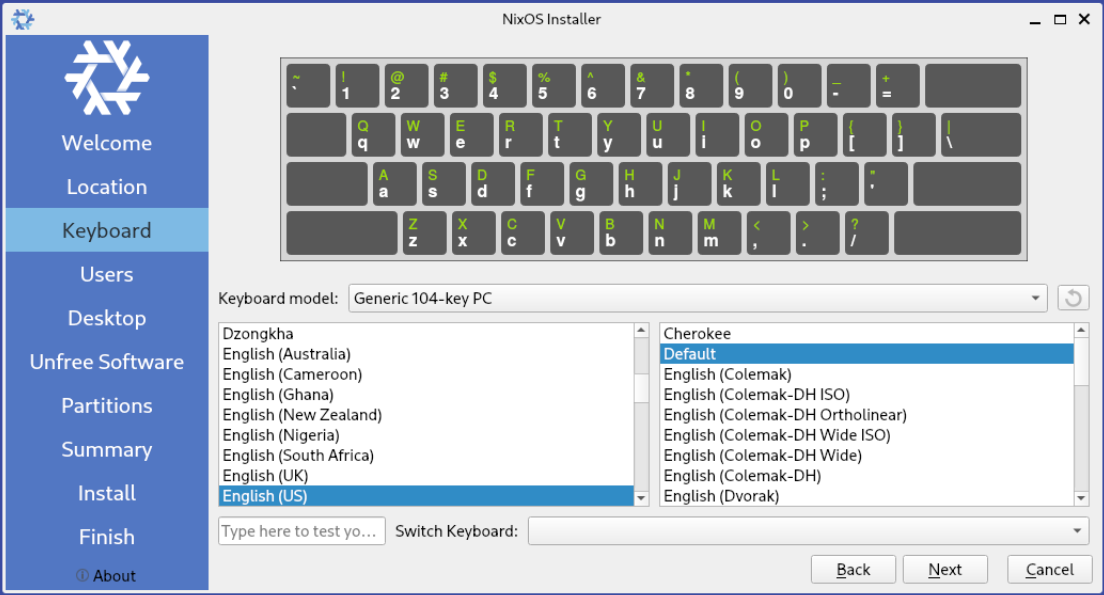
\includegraphics[width=0.95\textwidth]{images/nixos-23.11-keyboard.png}
				      \end{center}
				      \caption{NixOS 23.11 Keyboard}
			      \end{figure}

			\item Buat username dan password kemudian centang bagian "\textit{Use the
				      same password for the administrator account}".
			\item Untuk pilihan Desktop, pilih "No desktop" karena kita hanya butuh
			      akses SSH.
			\item Centang bagian "Allow Unfree Software".
			\item Buat skema partisi seperti berikut dengan tabel partisi GPT:
			      \begin{figure}[H]
				      \begin{center}
					      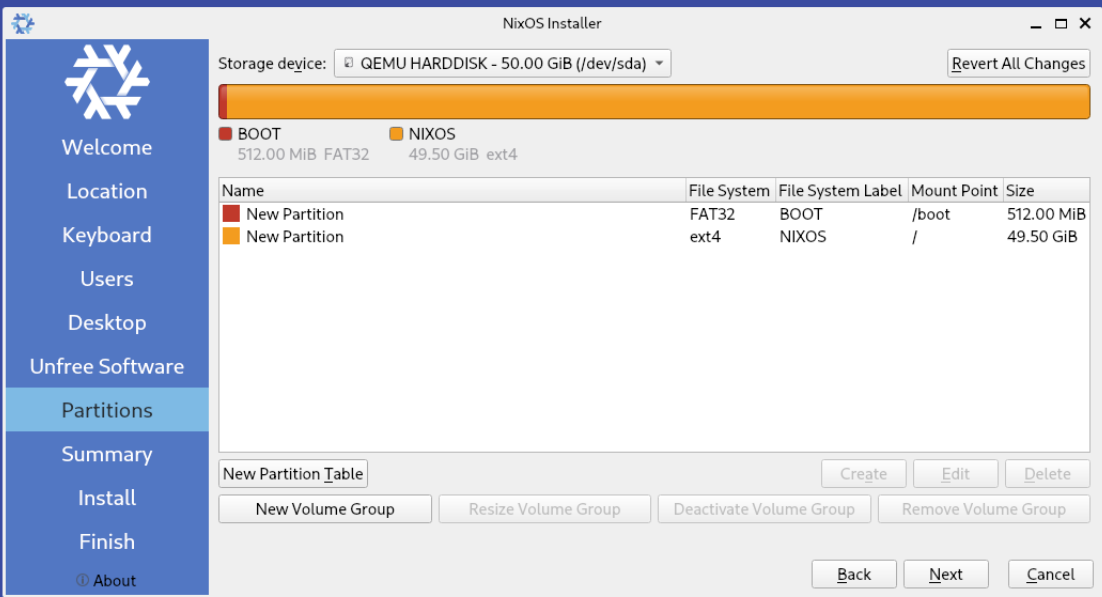
\includegraphics[width=0.95\textwidth]{images/nixos-install-partition.png}
				      \end{center}
				      \caption{NixOS Partition}
			      \end{figure}
			\item Lanjutkan hingga tahapan install.
			\item Ketika proses instalasi, NixOS akan \textit{stuck} tepat pada 46\%.
			      Ini karena NixOS sedang melakukan \textit{build derivation} untuk semua paket
			      yang diperlukan.
			\item Ketika instalasi sudah selesai, silahkan di \textit{restart}.
			\item Setelah instalasi, kita akan disambut dengan \textit{console login} seperti berikut:
			      \begin{figure}[H]
				      \begin{center}
					      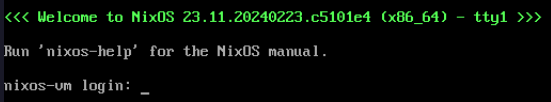
\includegraphics[width=0.95\textwidth]{images/nixos-23.11-tty.png}
				      \end{center}
				      \caption{NixOS 23.11 tty}
			      \end{figure}
		\end{enumerate}
	\end{adjustwidth}
	\subsubsection{Setup OS}
	\begin{adjustwidth}{20pt}{}
		Setelah itu, kita aktifkan SSH dan mematikan \textit{firewall} dengan
		menambahkan baris dibawah ini kedalam file /etc/nixos/configuration.nix:
		\begin{code}
			\begin{minted}{nix}
        services.openssh.enable = true;
        services.openssh.settings.PermitRootLogin = "yes";
        networking.firewall.enable = false;
      \end{minted}
			\caption{NixOS Enable SSH}
		\end{code}

		Kemudian, kita akan menambahkan beberapa paket untuk mempermudah dalam
		melakukan penelitian. Kita akan menginstall neovim sebagai \textit{text editor}
		dan tmux sebagai \textit{terminal multiplexer} untuk menjaga sesi SSH apabila koneksi
		SSH ke \textit{server} terputus.

		\begin{code}
			\begin{minted}{nix}
        environment.systemPackages = with pkgs; [
          neovim
          tmux
        ];
      \end{minted}
			\caption{NixOS Enable SSH}
		\end{code}

		Untuk target, tambahkan opsi berikut agar nixos-rebuild dapat menginstall
		systemd-boot dengan versi lebih rendah dari yang telah terinstall.
		\begin{code}
			\begin{minted}{nix}
        environment.sessionVariables = {NIXOS_INSTALL_BOOTLOADER = "1"; };
      \end{minted}
			\caption{NixOS install bootloader}
		\end{code}
		Setelah itu bisa diterapkan dengan perintah "sudo nixos-rebuild switch".
		Apabila tidak di spesifikasikan \textit{path}, maka secara \textit{default}
		akan mengarah ke /etc/nixos/configuration.nix.
	\end{adjustwidth}

	\subsection{Struktur Konfigurasi NixOS}
	\begin{adjustwidth}{20pt}{}

		Untuk struktur konfigurasi target yang digunakan adalah sebagai berikut:
		\begin{figure}[H]
			\centering
			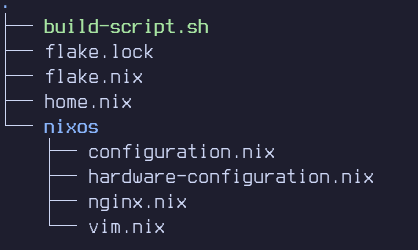
\includegraphics[width=0.6\textwidth]{images/nix-tree.png}
			\caption{Directory-tree}
		\end{figure}

		Dalam konfigurasi ini, flake.nix dan flake.lock diletakkan di parent
		directory yang memang menjadi basis untuk dieksekusinya perintah
		"nixos-rebuild switch -{}- flake .\#nixos-vm", dimana opsi -{}-flake sendiri
		terdiri dari flake-uri[\#hostname]

		\begin{code}
			\begin{minted}{nix}
        {
          inputs = {
            nixpkgs.url = "github:nixos/nixpkgs/nixos-23.11";
            home-manager = {
              url = "github:nix-community /home-manager/release-23.11";
              inputs.nixpkgs.follows = "nixpkgs";
            };
            testing-website = {
              url = "github:rizqirazkafi/testing-website";
              flake = false;
            };
          };
        }
      \end{minted}
			\caption{flake inputs}
		\end{code}

		Flake.nix berisi tiga inputs yang dimana terdiri dari nixpkgs, home-manager,
		dan testing-website. Hasil dari inputs tadi digunakan dalam output untuk
		sistem yang didefinisikan dalam nixosConfiguration dengan nixos-vm sebagai
		hostname dari sistem.

		\begin{code}[H]
			\begin{minted}{nix}
        {
          outputs = { self, nixpkgs, home-manager, ... }@inputs:
          let
          system = "x86_64-linux";
          pkgs = import nixpkgs {
            inherit system;
            config = { allowUnfree = true; };
          };
          in
          {
            nixosConfigurations = {
              nixos-vm = nixpkgs.lib.nixosSystem {
                specialArgs = { inherit inputs system pkgs; };
                modules = [ ./nixos/configuration.nix ];
              };
            };
          };
        }
      \end{minted}
			\caption{flake outputs}
		\end{code}

		Dengan flake, versi paket yang dihasilkan dalam output tidak akan berubah
		baik dari channel maupun hash. Ini dikarenakan, informasi tersebut disimpan
		dalam flake.lock. Dengan ini, sistem yang dihasilkan akan konsisten dan
		dapat disebut sebagai sistem yang \textit{reproducible}.

		Contoh konten flake.lock adalah sebagai berikut:

		\begin{code}
			\begin{minted}{json}
        {
          "nodes": {
            "nixpkgs": {
              "locked": {
                "lastModified": 1708702655,
                "narHash": "sha256-qxT5jSxxx",
                "owner": "nixos",
                "repo": "nixpkgs",
                "rev": "c5101e457206dd437330d283d6626944e28794b3",
                "type": "github"
              },
              "original": {
                "owner": "nixos",
                "ref": "nixos-23.11",
                "repo": "nixpkgs",
                "type": "github"
              },
            },
          }
        }
      \end{minted}
			\caption{nixpkgs lock di flake.lock}
		\end{code}

	\end{adjustwidth}
	\subsection{Konfigurasi inti configuration.nix}

	\begin{adjustwidth}{20pt}{}
		File configuration.nix berisikan konfigurasi sistem seperti \textit{system
			packages, services, user packages, ssh option, }dan lain-lain. File ini
		bisa dibilang merupakan file inti dari konfigurasi sistem secara menyeluruh
		dimana file inilah yang di evaluasi oleh nixos-rebuild. Semua module yang
		dibutuhkan sistem harus di referensikan dalam file ini agar konfigurasi
		dapat diterapkan ke sistem.
		Ini merupakan sebagian konten file configuration.nix yang digunakan pada
		penelitian ini:

		\begin{code}
			\begin{minted}{nix}
        {inputs, pkgs, ... }: {
          nixpkgs.config.allowUnfree = true;
          environment.systemPackages = with pkgs; [
            lazygit
            tmux
            vim
            neovim
            wget
            git
            home-manager
            htop
            ranger
            ripgrep
            ansible
          ];
          security.pam.enableSSHAgentAuth = true;
          security.pam.enableSSHAgentAuth = true;
          services.openssh = {
            enable = true;
            ports = [ 9005 ];
            settings.PasswordAuthentication = false;
          };
        }
      \end{minted}
		\end{code}
	\end{adjustwidth}
	\subsection{Home Manager}

	\begin{adjustwidth}{20pt}{}
		Untuk konfigurasi Home Manager, ada beberapa yang dimasukkan yaitu :
		\begin{enumerate}[nolistsep]
			\item userName dan userEmail git
			\item enableCompletion untuk BASH
		\end{enumerate}

		Berikut merupakan sebagian dari konfigurasi yang dipakai untuk penelitian ini:

		\begin{code}
			\begin{minted}{nix}
        {config, pkgs, inputs, ...}:
        {
          home.username = "rizqirazkafi";
          home.homeDirectory = "/home/rizqirazkafi";
          programs.git = {
            enable = true;
            userName = "Rizqirazkafi";
            userEmail = "rizqir****@gmail.com";
          };

          programs.bash = {
            enable = true;
            shellAliases = { ll = "ls -la"; };
            enableCompletion = true;
            initExtra = ''echo "Hello, what good shall I do today?"'';
          };
        }
      \end{minted}
			\caption{Konfigurasi home.nix untuk Home-Manager}
		\end{code}
	\end{adjustwidth}
	\subsection{Persiapan Lingkungan Ansible}
	\begin{adjustwidth}{20pt}{}
		Untuk persiapan lingkungan Ansible baik \textit{master} maupun target adalah
		sebagai berikut:
	\end{adjustwidth}
	\subsubsection{Download ISO dan konfigurasi VM}
	\begin{adjustwidth}{20pt}{}
		Download ISO Ubuntu 24.04 live server di \url{https://ubuntu.com} atau
		\url{https://kartolo.sby.datautama.net.id/ubuntu-cd}. Buat VM di Proxmox
		dengan konfigurasi yang sama dengan Lingkungan NixOS. Karena Ubuntu mendukung
		\textit{secure boot} sepenuhnya, kita tidak perlu mematikan \textit{secure boot}
		pada \textit{firmware setting} seperti NixOS.
		Ketika sudah \textit{booting}, maka akan muncul tampilan sebagai berikut:
		\newpage
		\begin{figure}[H]
			\begin{center}
				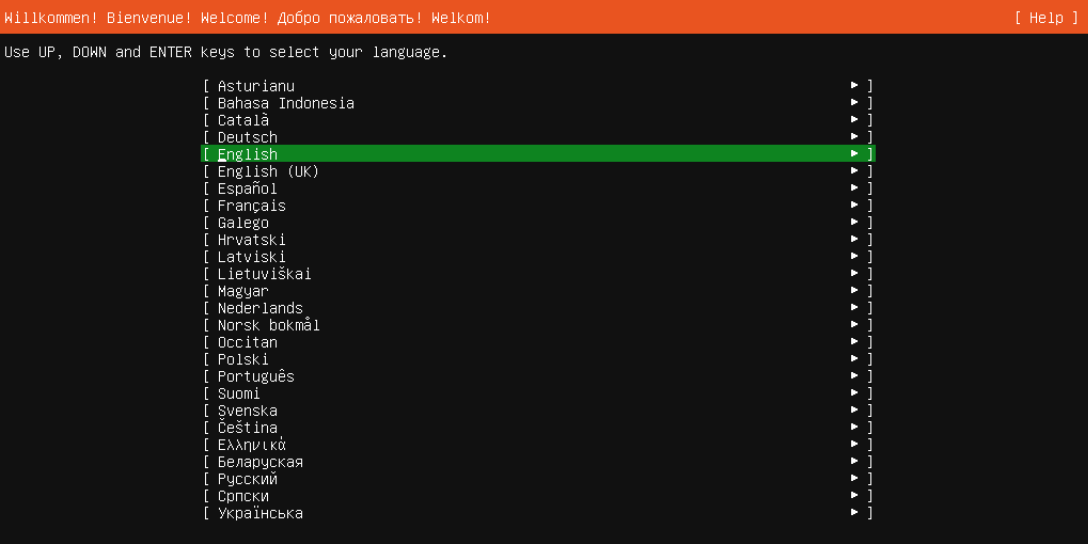
\includegraphics[width=0.95\textwidth]{images/ansible-nix-0.png}
			\end{center}
			\caption{Ubuntu 24.04 Live Server}
		\end{figure}

	\end{adjustwidth}
	\subsubsection{Instalasi}
	\begin{adjustwidth}{20pt}{}
		Kemudian kita masuk ke tahap instalasi Ubuntu Server sebagai berikut:
		\begin{enumerate}[nolistsep]
			\item Pilih bahasa dan keyboard yang diinginkan, penulis memilih Bahasa
			      Inggris dan \textit{layout} US.
			\item Pilih basis instalasi Ubuntu Server.
			\item Untuk IP, penulis menggunakan yang diberikan oleh DHCP server.
			\item Kosongkan proxy.
			\item Untuk \textit{mirror address} penulis menggunakan \url{https://id.archive.ubuntu.com/ubuntu}
			      \begin{figure}[H]
				      \begin{center}
					      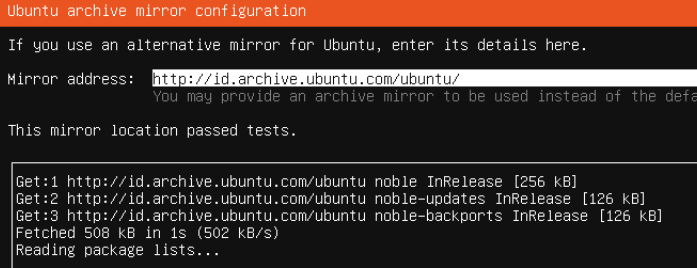
\includegraphics[width=0.95\textwidth]{images/ansible-nix-repo.png}
				      \end{center}
				      \caption{Repository Ubuntu}
			      \end{figure}
			      Pastikan \textit{repository} dapat dijangkau.
			\item Untuk \textit{disk} kita gunakan seluruhnya, untuk LVM dimatikan karena tidak dibutuhkan.
			      \begin{figure}[H]
				      \begin{center}
					      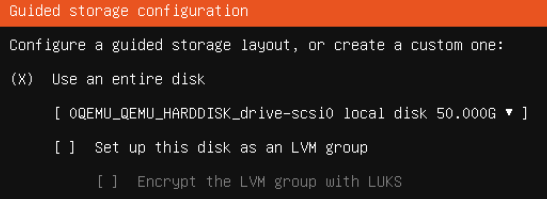
\includegraphics[width=0.95\textwidth]{images/ansible-nix-disk.png}
				      \end{center}
				      \caption{Ubuntu Server Disk}
			      \end{figure}
			      Hasilnya harusnya seperti ini:
			      \begin{figure}[H]
				      \begin{center}
					      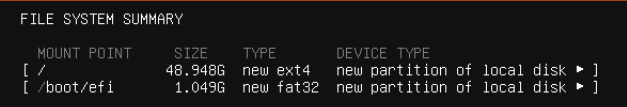
\includegraphics[width=0.95\textwidth]{images/ansible-nix-filesystem.png}
				      \end{center}
				      \caption{Ubuntu Server Disk Layout}
			      \end{figure}
			\item Kita skip Ubuntu Pro
			\item Kita tidak akan install SSH server pada saat instalasi
			\item Lanjut proses instalasi
			\item Apabila sudah selesai dan Ubuntu Server berhasil terinstall, maka hasilnya akan seperti ini:
			      \begin{figure}
				      \begin{center}
					      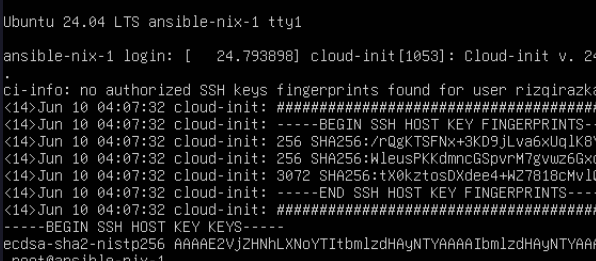
\includegraphics[width=0.95\textwidth]{images/ansible-nix-ready.png}
				      \end{center}
				      \caption{Ubuntu Server Telah terinstall}
			      \end{figure}
		\end{enumerate}
	\end{adjustwidth}
	\subsection{Konfigurasi Ansible}

	\begin{adjustwidth}{20pt}{}
		\hspace\parindent
		Untuk Ansible menggunakan konfigurasi yang lebih sederhana dengan menyalin
		file konfigurasi dari vim, tmux, ssh, dan nginx ke
		\textit{directory} konfigurasi sesuai Filesystem Hierarchial Standard
		(FHS). Untuk paket yang dibutuhkan di definisikan secara \textit{global
			packages} dimana paket di install untuk semua \textit{user}.

		Untuk \textit{Language Server Protocol} (LSP) \textit{server} akan
		ditangani oleh Lazy.nvim dan Mason agar terinstall secara otomatis
		saat Neovim dijalankan.

		Rincian konfigurasinya adalah sebagai berikut:

		\begin{code}
			\begin{minted}{yaml}
        - hosts: all
          become: yes
          become_user: root
          tasks:
          - name: install packages
            ansible.builtin.apt:
              pkg:
                - hello
                - neovim
                - tmux
                - vim
                - wget
                - ....
      \end{minted}
			\caption{Konfigurasi instalasi paket di Ansible}
		\end{code}

		\begin{code}
			\begin{minted}{yaml}
        - name: copy nginx default config
          ansible.builtin.copy:
            src: default
            dest: /etc/nginx/sites-enabled/default
        - name: copy php8.3-fpm config
          ansible.builtin.copy:
            src: php-demo.conf
            dest: /etc/php/8.3/fpm/pool.d
      \end{minted}
			\caption{Salin konfigurasi paket dan services ke target}
		\end{code}

		\begin{code}
			\begin{minted}{yaml}
        - name: enable nginx
        ansible.builtin.service:
          name: nginx
          state: restarted
      \end{minted}
			\caption{Restart service menggunakan Ansible}
		\end{code}

		Maka dengan kedua \textit{tool} Manajemen Konfigurasi inilah telah tercapai sistem
		GNU/Linux yang terdeklarasi dimana sistem terdeklarasikan dalam bentuk
		file-file konfigurasi.
	\end{adjustwidth}
\end{adjustwidth}
\newpage
\section{Pengujian}
\begin{adjustwidth}{20pt}{}
	\hspace\parindent
	Tahap pengujian yang dilakukan dalam penelitian ini dimaksudkan untuk mengetahui
	waktu eksekusi yang dibutuhkan dari Ansible dan NixOS untuk menerapkan manajemen
	konfigurasi yang telah dibuat. Pengujian dilakukan dengan menggunakan perintah
	"\textit{time}" pada eksekusi setiap kali dijalankan perintah untuk penerapan manajemen
	konfigurasi.

	Pengujian berikutnya ialah menguji apakah baik Ansible maupun NixOS bersifat
	deklaratif dalam penerapannya menggunakan perbandingan dari apa yang telah
	di deklarasikan di konfigurasi dengan hasil akhir pada sistem.
	\subsection{Pasca Install}
	\begin{adjustwidth}{20pt}{}
		Pengujian dilakukan dengan menjalankan Ansible Playbook dan nixos-rebuild
		ke dua Virtual Machine yang baru saja di install. Tidak ada konfigurasi
		tambahan selain konfigurasi untuk IP menggunakan NetworkManager dan SSH.
		Masing-masing sistem juga berjalan di mode shell tanpa GUI. Pengujian ini
		akan dijalankan sebanyak tiga kali.
	\end{adjustwidth}

	\subsubsection{NixOS tanpa cache}
	\begin{adjustwidth}{20pt}{}
		Pada percobaan ini, \textit{master} akan mengunduh semua \textit{binary}
		dan \textit{dependency} kemudian akan melakukan \textit{build} berdasarkan
		\textit{derivation} yang telah di definisikan oleh nixpkgs. Hasil dari
		\textit{derivation} berupa \textit{closure} yang disalin ke target. Karena
		nixos-rebuild tidak dapat berjalan secara paralel, maka percobaan dilakukan secara bergantian
		untuk masing-masing target. Setelah nixos-rebuild menyalin \textit{closure}
		ke target, maka waktu eksekusi telah didapat.Setelah waktu eksekusi
		didapat, baik VM untuk target dan \textit{master} akan dikembalikan ke
		\textit{snapshot} sebelum dijalankannya nixos-rebuild. Percobaan dilakukan
		tiga kali untuk masing-masing target.
		\begin{figure}[H]
			\begin{center}
				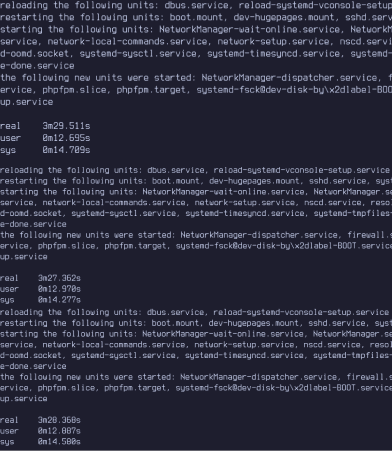
\includegraphics[width=0.8\textwidth]{images/nix-target/nix-pasca-install-25-com.png}
			\end{center}
			\caption{nixos-rebuild first target tanpa cache}
		\end{figure}
		\begin{figure}[H]
			\begin{center}
				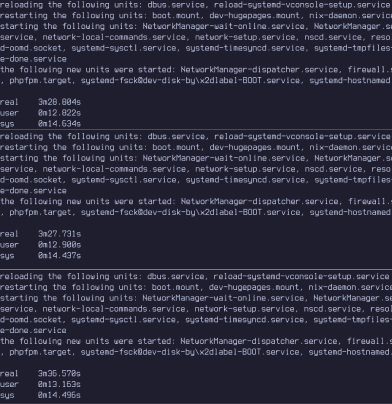
\includegraphics[width=0.8\textwidth]{images/nix-target/nix-pasca-install-26-com.png}
			\end{center}
			\caption{nixos-rebuild second target tanpa cache}
		\end{figure}

	\end{adjustwidth}
	\begin{table}[H]
		\caption{nixos-rebuild first target tanpa cache}
		\begin{center}
			\begin{tabular}[c]{|c|c|c|c|}
				\hline
				\multicolumn{1}{|c|}{\textbf{Iterasi ke-}} &
				\multicolumn{1}{c|}{\textbf{real}}         &
				\multicolumn{1}{c|}{\textbf{user}}         &
				\multicolumn{1}{c|}{\textbf{sys}}                                              \\
				\hline
				1                                          & 3m29.511s & 0m12.695s & 0m14.709s \\
				\hline
				2                                          & 3m27.362s & 0m12.970s & 0m14.277s \\
				\hline
				3                                          & 3m28.368s & 0m12.887s & 0m14.580s \\
				\hline
			\end{tabular}
		\end{center}
	\end{table}
	\vspace{-5mm}
	\begin{table}[H]
		\caption{nixos-rebuild second target tanpa cache}
		\begin{center}
			\begin{tabular}[c]{|c|c|c|c|}
				\hline
				\multicolumn{1}{|c|}{\textbf{Iterasi ke-}} &
				\multicolumn{1}{c|}{\textbf{real}}         &
				\multicolumn{1}{c|}{\textbf{user}}         &
				\multicolumn{1}{c|}{\textbf{sys}}                                              \\
				\hline
				1                                          & 3m28.804s & 0m12.822s & 0m14.634s \\
				\hline
				2                                          & 3m27.731s & 0m12.900s & 0m14.437s \\
				\hline
				3                                          & 3m36.570s & 0m13.163s & 0m14.496s \\
				\hline
			\end{tabular}
		\end{center}
	\end{table}
	\subsubsection{NixOS dengan Cache}
	\begin{adjustwidth}{20pt}{}
		\hspace\parindent Pada percobaan ini, nixos-rebuild tidak lagi perlu mengunduh binary karena sudah
		di \textit{build} di \textit{master}. \textit{Master} hanya perlu menyalin \textit{closure}
		ke target. Percobaan dilakukan sebanyak tiga kali, dimana sebelum percobaan, VM
		dan target akan di \textit{snapshot} sehingga dapat kembali ke \textit{state}
		sebelum diterapkannya konfigurasi.

		\begin{figure}[H]
			\begin{center}
				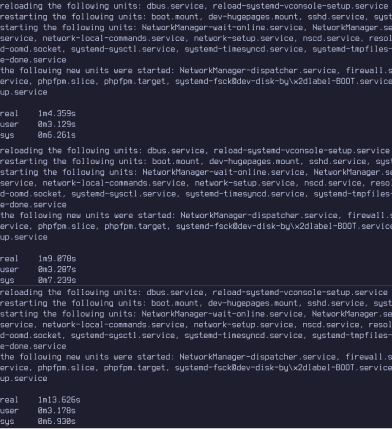
\includegraphics[width=0.8\textwidth]{images/nix-target/nix-pasca-cache-25-com.png}
			\end{center}
			\caption{nixos-rebuild first target dengan cache}
		\end{figure}

		\newpage
		\begin{figure}[H]
			\begin{center}
				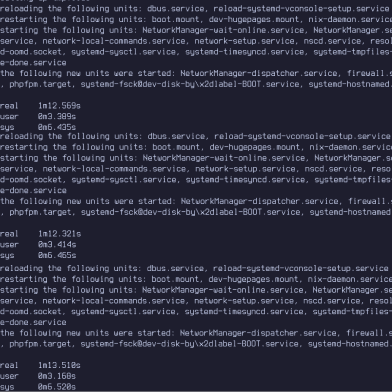
\includegraphics[width=0.8\textwidth]{images/nix-target/nix-pasca-cache-26-com.png}
			\end{center}
			\caption{nixos-rebuild second target dengan cache}
		\end{figure}

		\begin{table}[H]
			\caption{nixos-rebuild first target dengan cache}
			\begin{center}
				\begin{tabular}[c]{|c|c|c|c|}
					\hline
					\multicolumn{1}{|c|}{\textbf{Iterasi ke-}} &
					\multicolumn{1}{c|}{\textbf{real}}         &
					\multicolumn{1}{c|}{\textbf{user}}         &
					\multicolumn{1}{c|}{\textbf{sys}}                                            \\
					\hline
					1                                          & 1m4.359s  & 0m3.129s & 0m6.261s \\
					\hline
					2                                          & 1m9.078s  & 0m3.287s & 0m7.239s \\
					\hline
					3                                          & 1m13.626s & 0m3.178s & 0m6.930s \\
					\hline
				\end{tabular}
			\end{center}
		\end{table}
		\vspace{-5mm}
		\begin{table}[H]
			\caption{nixos-rebuild second target}
			\begin{center}
				\begin{tabular}[c]{|c|c|c|c|}
					\hline
					\multicolumn{1}{|c|}{\textbf{Iterasi ke-}} &
					\multicolumn{1}{c|}{\textbf{real}}         &
					\multicolumn{1}{c|}{\textbf{user}}         &
					\multicolumn{1}{c|}{\textbf{sys}}                                            \\
					\hline
					1                                          & 1m12.569s & 0m3.389s & 0m6.435s \\
					\hline
					2                                          & 1m12.321s & 0m3.414s & 0m6.465s \\
					\hline
					3                                          & 1m13.510s & 0m3.168s & 0m6.520s \\
					\hline
				\end{tabular}
			\end{center}
		\end{table}
		Patut diketahui bahwa kecepatan untuk menyalin \textit{closure} dari \textit{master}
		ke target bergantung kepada koneksi antara keduanya. Dalam percobaan ini,
		antara \textit{master} dengan target terkoneksi dengan \textit{bandwidth} sebesar
		1 Gbps.
	\end{adjustwidth}
	\subsubsection{Ansible Single Target}
	\begin{adjustwidth}{20pt}{}
		Pada percobaan ini, dijalankan menggunakan perintah ansible-playbook dengan
		satu target pada satu waktu. Total target yang di tuju adalah dua dengan
		setiap kali dijalankan, VM target akan dikembalikan ke \textit{snapshot}
		yang berisi \textit{state} sebelum ansible-playbook diterapkan ke target.
		Percobaan ini dilakukan tiga kali di masing-masing target.
		\begin{figure}[H]
			\begin{center}
				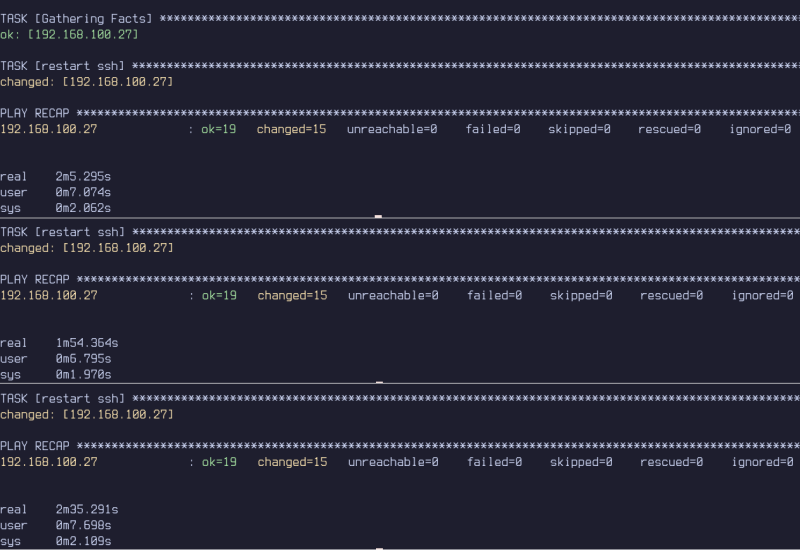
\includegraphics[width=\textwidth]{images/ansible/single/ansible-pasca-27-com.png}
			\end{center}
			\caption{Ansible first target pasca install}
		\end{figure}
		\newpage
		\begin{figure}[H]
			\begin{center}
				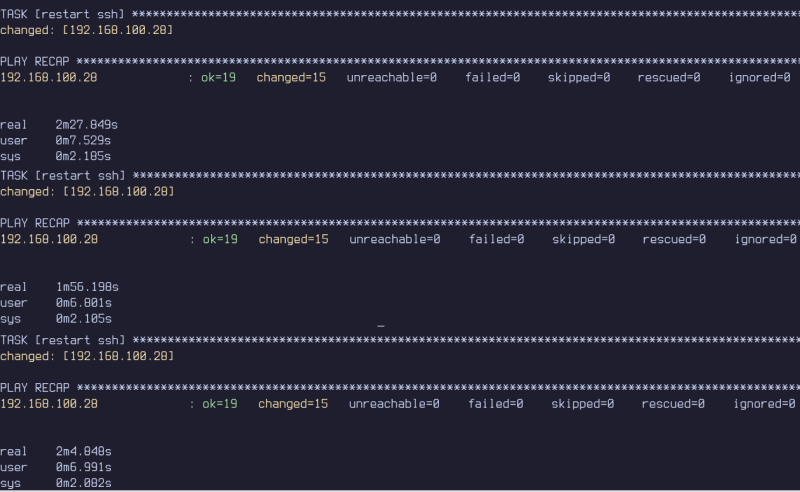
\includegraphics[width=\textwidth]{images/ansible/single/ansible-pasca-28-com.png}
			\end{center}
			\caption{Ansible second target pasca install}
		\end{figure}

		\begin{table}[H]
			\caption{Ansible first target pasca install}
			\begin{center}
				\begin{tabular}[c]{|c|c|c|c|}
					\hline
					\multicolumn{1}{|c|}{\textbf{Iterasi ke-}} &
					\multicolumn{1}{c|}{\textbf{real}}         &
					\multicolumn{1}{c|}{\textbf{user}}         &
					\multicolumn{1}{c|}{\textbf{sys}}                                            \\
					\hline
					1                                          & 2m5.295s  & 0m7.074s & 0m2.062s \\
					\hline
					2                                          & 1m54.364s & 0m6.795s & 0m1.970s \\
					\hline
					3                                          & 2m35.291s & 0m7.698s & 0m2.109s \\
					\hline
				\end{tabular}
			\end{center}
		\end{table}
		\vspace{-5mm}

		\begin{table}[H]
			\caption{ansible second target pasca install}
			\begin{center}
				\begin{tabular}[c]{|c|c|c|c|}
					\hline
					\multicolumn{1}{|c|}{\textbf{Iterasi ke-}} &
					\multicolumn{1}{c|}{\textbf{real}}         &
					\multicolumn{1}{c|}{\textbf{user}}         &
					\multicolumn{1}{c|}{\textbf{sys}}                                             \\
					\hline
					1                                          & 2m32.026s & 0m10.997s & 0m3.703s \\
					\hline
					2                                          & 3m19.488s & 0m12.124s & 0m3.995s \\
					\hline
					3                                          & 4m23.604s & 0m13.486s & 0m4.481s \\
					\hline
				\end{tabular}
			\end{center}
		\end{table}
	\end{adjustwidth}
	\subsubsection{Ansible Multi Target}
	\begin{adjustwidth}{20pt}{}
		Pada percobaan ini, dijalankan menggunakan perintah ansible-playbook dengan dua
		target secara paralel. Setiap kali sebelum ansible-playbook diterapkan ke target,
		target akan dikembalikan ke \textit{snapshot} sebelum ansible-playbook diterapkan.
		\newpage
		\begin{center}
			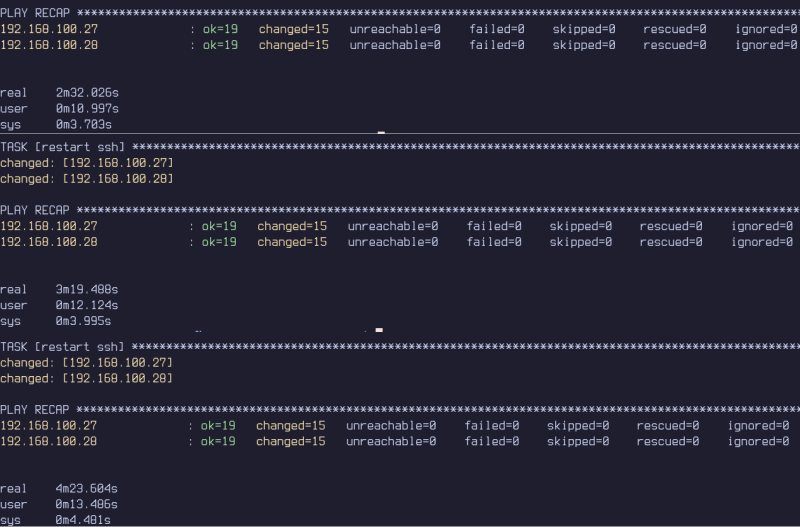
\includegraphics[width=\textwidth]{images/ansible/multi/ansible-pasca-multi-com.png}
		\end{center}
		\caption{Ansible multi target pasca install}
		\end{figure}
		\begin{table}[H]
			\caption{ansible multi target pasca install}
			\begin{center}
				\begin{tabular}[c]{|c|c|c|c|}
					\hline
					\multicolumn{1}{|c|}{\textbf{Iterasi ke-}} &
					\multicolumn{1}{c|}{\textbf{real}}         &
					\multicolumn{1}{c|}{\textbf{user}}         &
					\multicolumn{1}{c|}{\textbf{sys}}                                            \\
					\hline
					1                                          & 2m12.327s & 0m9.902s & 0m3.188s \\
					\hline
					2                                          & 1m56.784s & 0m9.654s & 0m3.147s \\
					\hline
					3                                          & 2m2.801s  & 0m9.889s & 0m2.932s \\
					\hline
				\end{tabular}
			\end{center}
		\end{table}
	\end{adjustwidth}
	\subsection{Penerapan ulang setelah pasca install.}
	\begin{adjustwidth}{20pt}{}
		Pengujian ini dilakukan dengan cara menjalankan Ansible Playbook dan nixos-rebuild
		setelah pengujian Pasca Install tanpa perubahan apapun pada file konfigurasi. Pengujian ini
		akan dijalankan sebanyak tiga kali.
	\end{adjustwidth}
	\subsubsection{NixOS}
	\begin{adjustwidth}{20pt}{}
		Untuk NixOS, dijalankan perintah nixos-rebuild dengan dua target. Masing-masing target
		dijalankan sebanyak tiga kali tanpa perlu mengembalikan VM ke kondisi sebelumnya dengan
		\textit{snapshot}. Berikut hasil pengujiannya:
		\begin{figure}[H]
			\begin{center}
				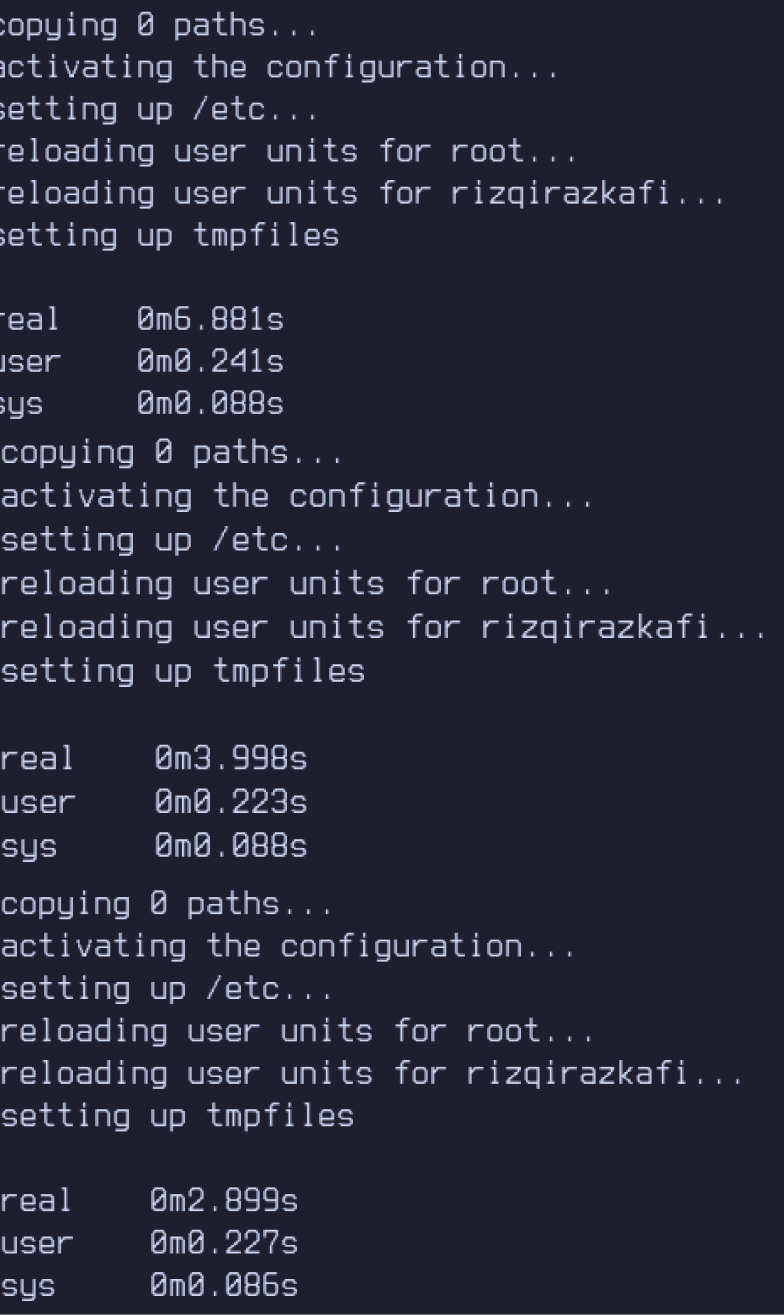
\includegraphics[width=0.8\textwidth]{images/nix-target/nix-rerun-25-com.png}
			\end{center}
			\caption{nixos-rebuild first target pasca install rerun}
		\end{figure}

		\begin{figure}[H]
			\begin{center}
				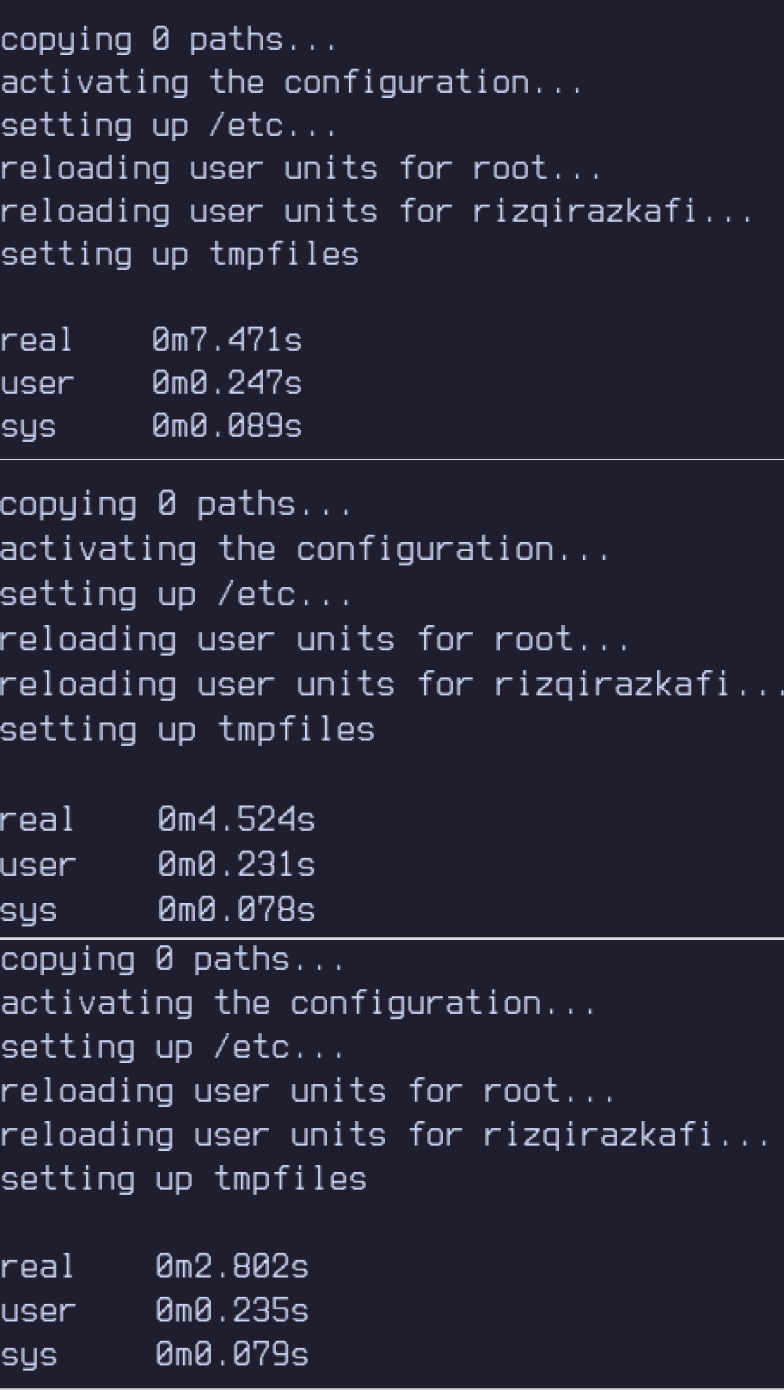
\includegraphics[width=0.8\textwidth]{images/nix-target/nix-rerun-26-com.png}
			\end{center}
			\caption{nixos-rebuild second target pasca install rerun}
		\end{figure}

	\end{adjustwidth}
	\begin{table}[H]
		\caption{nixos-rebuild first target pasca install rerun}
		\begin{center}
			\begin{tabular}[c]{|c|c|c|c|}
				\hline
				\multicolumn{1}{|c|}{\textbf{Iterasi ke-}} &
				\multicolumn{1}{c|}{\textbf{real}}         &
				\multicolumn{1}{c|}{\textbf{user}}         &
				\multicolumn{1}{c|}{\textbf{sys}}                                           \\
				\hline
				1                                          & 0m6.881s & 0m0.241s & 0m0.088s \\
				\hline
				2                                          & 0m3.998s & 0m0.223s & 0m0.088s \\
				\hline
				3                                          & 0m2.899s & 0m0.227s & 0m0.086s \\
				\hline
			\end{tabular}
		\end{center}
	\end{table}
	\vspace{-5mm}
	\begin{table}[H]
		\caption{nixos-rebuild second target pasca install rerun}
		\begin{center}
			\begin{tabular}[c]{|c|c|c|c|}
				\hline
				\multicolumn{1}{|c|}{\textbf{Iterasi ke-}} &
				\multicolumn{1}{c|}{\textbf{real}}         &
				\multicolumn{1}{c|}{\textbf{user}}         &
				\multicolumn{1}{c|}{\textbf{sys}}                                           \\
				\hline
				1                                          & 0m7.471s & 0m0.247s & 0m0.089s \\
				\hline
				2                                          & 0m4.524s & 0m0.231s & 0m0.078s \\
				\hline
				3                                          & 0m2.802s & 0m0.235s & 0m0.079s \\
				\hline
			\end{tabular}
		\end{center}
	\end{table}
	\subsubsection{Ansible single target}
	\begin{adjustwidth}{20pt}{}
		Untuk percobaan Ansible \textit{single target}, perintah ansible-playbook dijalankan
		ke satu target dalam satu waktu. Ini digunakan untuk mendapatkan hasil perbandingan
		yang setara dengan nixos-rebuild yang hanya mampu mengkonfigurasi satu target
		dalam satu waktu.
	\end{adjustwidth}
	\begin{figure}[H]
		\begin{center}
			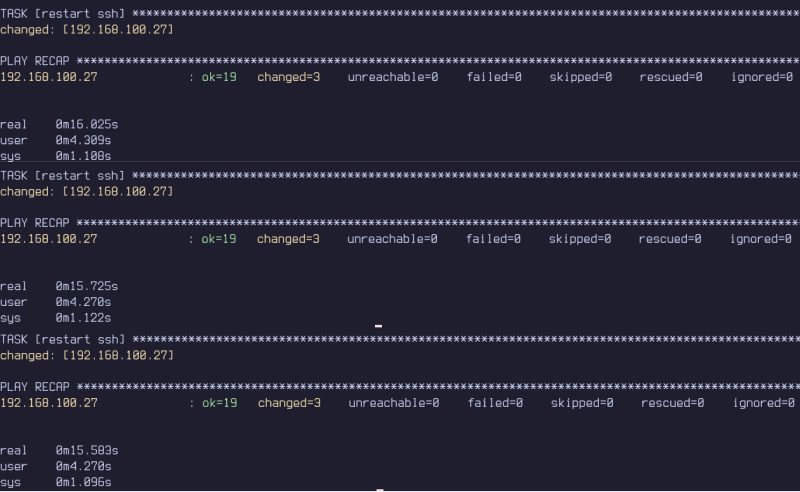
\includegraphics[width=0.8\textwidth]{images/ansible/single/ansible-rerun-27-com.png}
		\end{center}
		\caption{Ansible first target rerun}
	\end{figure}
	\begin{figure}[H]
		\begin{center}
			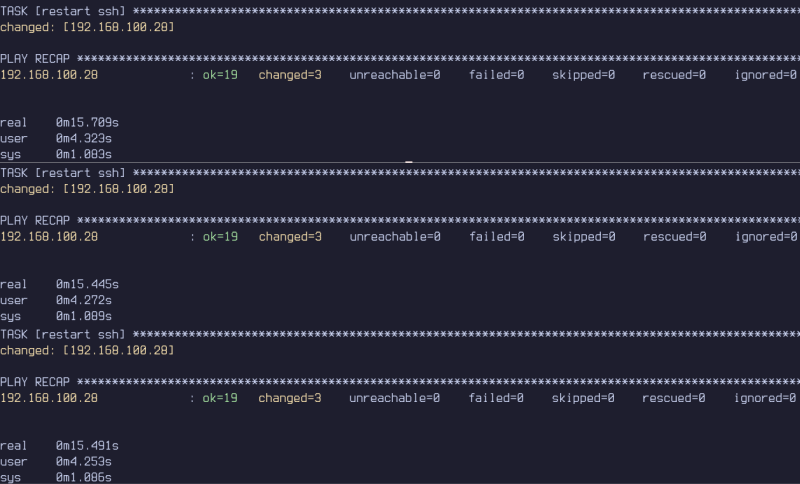
\includegraphics[width=0.8\textwidth]{images/ansible/single/ansible-rerun-28-com.png}
		\end{center}
		\caption{Ansible second target rerun}
	\end{figure}

	\begin{table}[H]
		\caption{Ansible first target rerun}
		\begin{center}
			\begin{tabular}[c]{|c|c|c|c|}
				\hline
				\multicolumn{1}{|c|}{\textbf{Iterasi ke-}} &
				\multicolumn{1}{c|}{\textbf{real}}         &
				\multicolumn{1}{c|}{\textbf{user}}         &
				\multicolumn{1}{c|}{\textbf{sys}}                                            \\
				\hline
				1                                          & 0m16.025s & 0m4.309s & 0m1.108s \\
				\hline
				2                                          & 0m15.725s & 0m4.270s & 0m1.122s \\
				\hline
				3                                          & 0m15.583s & 0m4.270s & 0m1.096s \\
				\hline
			\end{tabular}
		\end{center}
	\end{table}
	\vspace{-5mm}
	\begin{table}[H]
		\caption{Ansible second target rerun}
		\begin{center}
			\begin{tabular}[c]{|c|c|c|c|}
				\hline
				\multicolumn{1}{|c|}{\textbf{Iterasi ke-}} &
				\multicolumn{1}{c|}{\textbf{real}}         &
				\multicolumn{1}{c|}{\textbf{user}}         &
				\multicolumn{1}{c|}{\textbf{sys}}                                            \\
				\hline
				1                                          & 0m15.709s & 0m4.323s & 0m1.083s \\
				\hline
				2                                          & 0m15.445s & 0m4.272s & 0m1.089s \\
				\hline
				3                                          & 0m15.491s & 0m4.253s & 0m1.086s \\
				\hline
			\end{tabular}
		\end{center}
	\end{table}
	\subsubsection{Ansible multi target}
	\begin{adjustwidth}{20pt}{}
		Untuk percobaan Ansible \textit{multi target}, perintah ansible-playbook dijalankan
		ke dua target secara paralel. Berikut merupakan hasil dari percobaan Ansible \textit{multi target}:
	\end{adjustwidth}
	\newpage
	\begin{figure}
		\begin{center}
			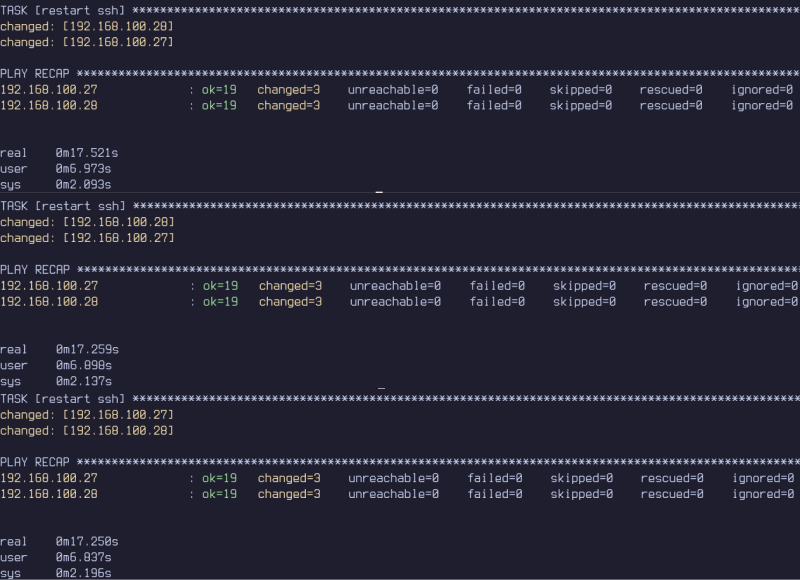
\includegraphics[width=0.8\textwidth]{images/ansible/multi/ansible-rerun-multi-com.png}
		\end{center}
		\caption{Ansible multi target rerun}
	\end{figure}

	\begin{table}[H]
		\caption{Ansible multi target}
		\begin{center}
			\begin{tabular}[c]{|c|c|c|c|}
				\hline
				\multicolumn{1}{|c|}{\textbf{Iterasi ke-}} &
				\multicolumn{1}{c|}{\textbf{real}}         &
				\multicolumn{1}{c|}{\textbf{user}}         &
				\multicolumn{1}{c|}{\textbf{sys}}                                            \\
				\hline
				1                                          & 0m17.521s & 0m6.973s & 0m2.093s \\
				\hline
				2                                          & 0m17.259s & 0m6.898s & 0m2.137s \\
				\hline
				3                                          & 0m17.250s & 0m6.837s & 0m2.196s \\
				\hline
			\end{tabular}
		\end{center}
	\end{table}
	\subsection{Penambahan Paket}
	\begin{adjustwidth}{20pt}{}
		Pengujian dilakukan dengan menambahkan paket tambahan yaitu Go compiler.
		Pengujian ini akan dilakukan tiga kali dengan satu kali perubahan pada file
		konfigurasi.
	\end{adjustwidth}
	\subsubsection{NixOS tanpa cache}
	\begin{adjustwidth}{20pt}{}
		Untuk NixOS, penambahan konfigurasi dilakukan pada file configuration.nix, pada
		bagian environment.systemPackages sebagai berikut:
		\begin{code}
			\begin{minted}{nix}
        environment.systemPackages = with pkgs; [
          go
        ];
      \end{minted}
			\caption{NixOS Go Package}
		\end{code}
		Pengujian dilakukan dengan pertama mengembalikan kondisi sistem baik
		\textit{master} maupun target ke konfigurasi setelah pasca install,
		kemudian menambahkan "go" kedalam konfigurasi. Ini dimaksudkan agar NixOS tidak
		menyimpan cache hasil \textit{build} untuk paket Go. Konfigurasi kemudian
		diterapkan dengan nixos-rebuild oleh \textit{master} ke target. Setelah
		master melakukan \textit{build}, master kemudian menyalin hasilnya ke
		target. Percobaan ini dilakukan berulang sebanyak tiga kali per target.
	\end{adjustwidth}
	\begin{figure}[H]
		\begin{center}
			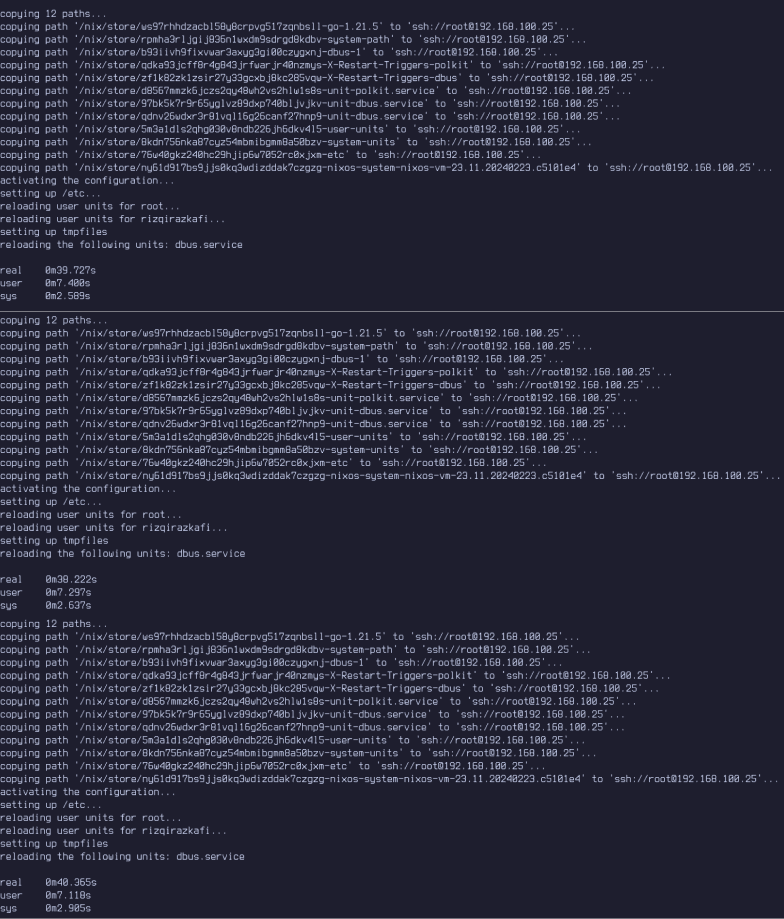
\includegraphics[width=0.8\textwidth]{images/nix-target/nix-go-25-com.png}
		\end{center}
		\caption{nixos-rebuild first target install Go}
	\end{figure}
	\newpage
	\begin{figure}[H]
		\begin{center}
			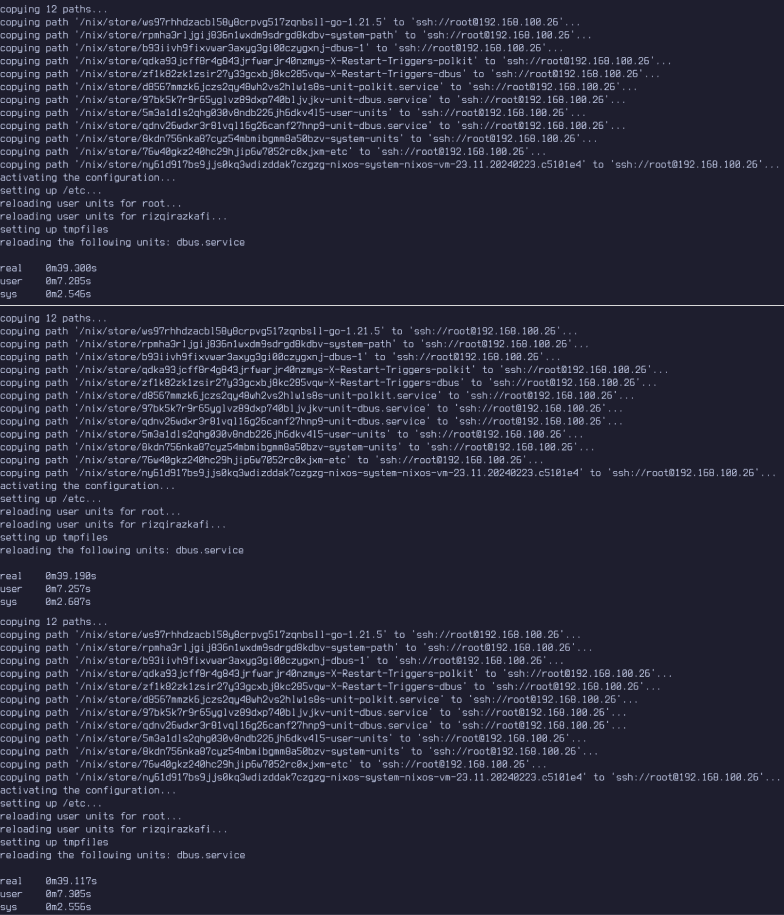
\includegraphics[width=0.8\textwidth]{images/nix-target/nix-go-26-com.png}
		\end{center}
		\caption{nixos-rebuild second target install Go}
	\end{figure}
	\begin{table}[H]
		\caption{nixos-rebuild first target}
		\begin{center}
			\begin{tabular}[c]{|c|c|c|c|}
				\hline
				\multicolumn{1}{|c|}{\textbf{Iterasi ke-}} &
				\multicolumn{1}{c|}{\textbf{real}}         &
				\multicolumn{1}{c|}{\textbf{user}}         &
				\multicolumn{1}{c|}{\textbf{sys}}                                            \\
				\hline
				1                                          & 0m39.727s & 0m7.400s & 0m2.589s \\
				\hline
				2                                          & 0m38.222s & 0m7.297s & 0m2.637s \\
				\hline
				3                                          & 0m40.365s & 0m7.118s & 0m2.905s \\
				\hline
			\end{tabular}
		\end{center}
	\end{table}
	\vspace{-5mm}
	\newpage
	\begin{table}[H]
		\caption{nixos-rebuild second target}
		\begin{center}
			\begin{tabular}[c]{|c|c|c|c|}
				\hline
				\multicolumn{1}{|c|}{\textbf{Iterasi ke-}} &
				\multicolumn{1}{c|}{\textbf{real}}         &
				\multicolumn{1}{c|}{\textbf{user}}         &
				\multicolumn{1}{c|}{\textbf{sys}}                                            \\
				\hline
				1                                          & 0m39.300s & 0m7.285s & 0m2.546s \\
				\hline
				2                                          & 0m39.190s & 0m7.257s & 0m2.687s \\
				\hline
				3                                          & 0m39.117s & 0m7.305s & 0m2.556s \\
				\hline
			\end{tabular}
		\end{center}
	\end{table}
	\subsubsection{NixOS dengan cache}
	\begin{adjustwidth}{20pt}{}
		Pada percobaan ini, NixOS telah melakukan \textit{build} untuk paket GO dan
		nixos-rebuild hanya perlu menyalin hasilnya ke target. Dari percobaan tersebut,
		didapatkan hasil sebagai berikut dengan pertimbangan \textit{bandwidth} dari
		\textit{master} ke target adalah 1 Gbps.
	\end{adjustwidth}
	\newpage
	\begin{figure}[H]
		\begin{center}
			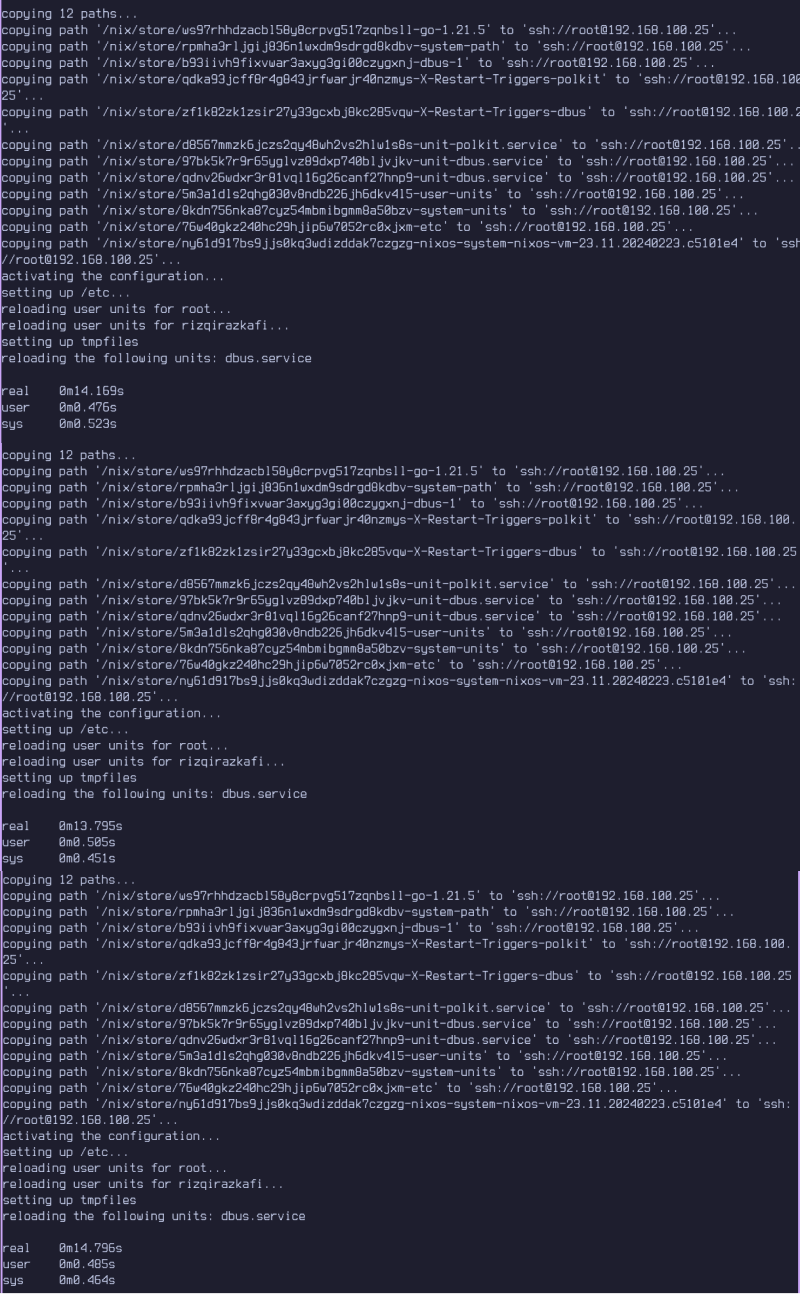
\includegraphics[width=0.8\textwidth]{images/nix-target/nix-go-cache-25-com.png}
		\end{center}
		\caption{nixos-rebuild first target install Go cache}
	\end{figure}

	\begin{figure}[H]
		\begin{center}
			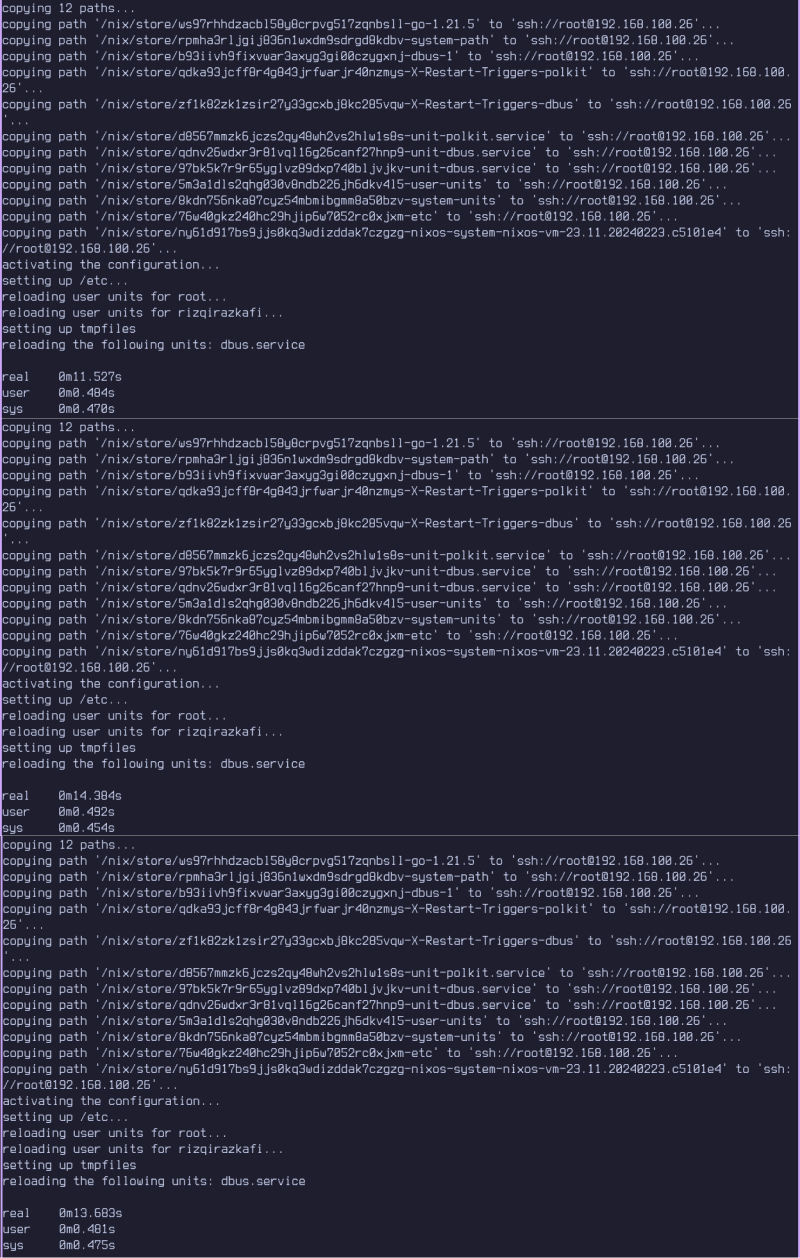
\includegraphics[width=0.8\textwidth]{images/nix-target/nix-go-cache-26-com.png}
		\end{center}
		\caption{nixos-rebuild second target install Go cache}
	\end{figure}

	\begin{table}[H]
		\caption{nixos-rebuild first target install Go cache}
		\begin{center}
			\begin{tabular}[c]{|c|c|c|c|}
				\hline
				\multicolumn{1}{|c|}{\textbf{Iterasi ke-}} &
				\multicolumn{1}{c|}{\textbf{real}}         &
				\multicolumn{1}{c|}{\textbf{user}}         &
				\multicolumn{1}{c|}{\textbf{sys}}                                            \\
				\hline
				1                                          & 0m14.169s & 0m0.476s & 0m0.523s \\
				\hline
				2                                          & 0m13.795s & 0m0.505s & 0m0.451s \\
				\hline
				3                                          & 0m14.796s & 0m0.485s & 0m0.464s \\
				\hline
			\end{tabular}
		\end{center}
	\end{table}
	\vspace{-5mm}
	\begin{table}[H]
		\caption{nixos-rebuild second target install Go cache}
		\begin{center}
			\begin{tabular}[c]{|c|c|c|c|}
				\hline
				\multicolumn{1}{|c|}{\textbf{Iterasi ke-}} &
				\multicolumn{1}{c|}{\textbf{real}}         &
				\multicolumn{1}{c|}{\textbf{user}}         &
				\multicolumn{1}{c|}{\textbf{sys}}                                            \\
				\hline
				1                                          & 0m11.527s & 0m0.484s & 0m0.470s \\
				\hline
				2                                          & 0m14.384s & 0m0.492s & 0m0.454s \\
				\hline
				3                                          & 0m13.683s & 0m0.481s & 0m0.475s \\
				\hline
			\end{tabular}
		\end{center}
	\end{table}
	\subsubsection{Ansible single target}
	\begin{adjustwidth}{20pt}{}
		Pada percobaan Ansible \textit{single target}, penambahan paket "GO" di definisikan
		dalam file yml yang digunakan seperti berikut:
		\begin{code}
			\begin{minted}{yaml}
      - name: install go
        ansible.builtin.apt:
          pkg:
            - golang-go
          state: present
      \end{minted}
			\caption{Ansible penambahan paket GO}
		\end{code}
		Pada konfigurasi tersebut, "state: absent" digunakan untuk memberitahu
		Ansible untuk memastikan apakah paket "golang-go" benar-benar ada pada
		sistem. Percobaan ini dilakukan sebanyak tiga kali untuk masing-masing
		target dan setiap sebelum percobaan kondisi VM akan dikembalikan ke
		\textit{snapshot} pasca install.
	\end{adjustwidth}
	\newpage
	\begin{figure}[H]
		\begin{center}
			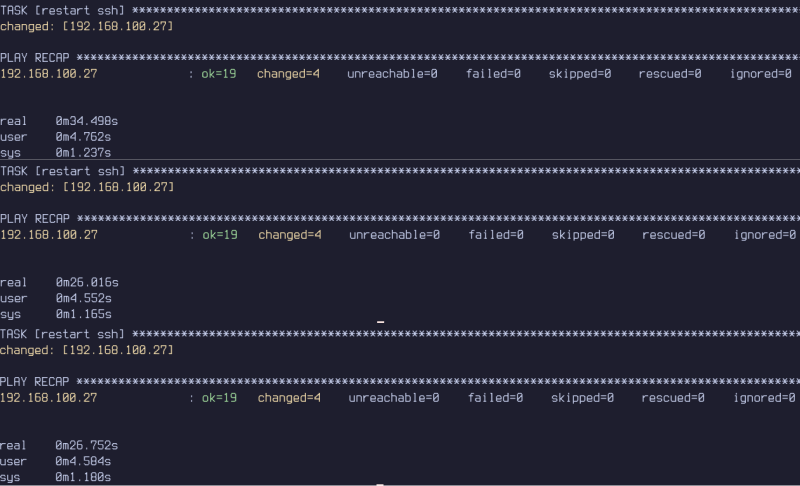
\includegraphics[width=0.8\textwidth]{images/ansible/single/ansible-go-27-com.png}
		\end{center}
		\caption{Ansible first target install Go}
	\end{figure}
	\begin{figure}[H]
		\begin{center}
			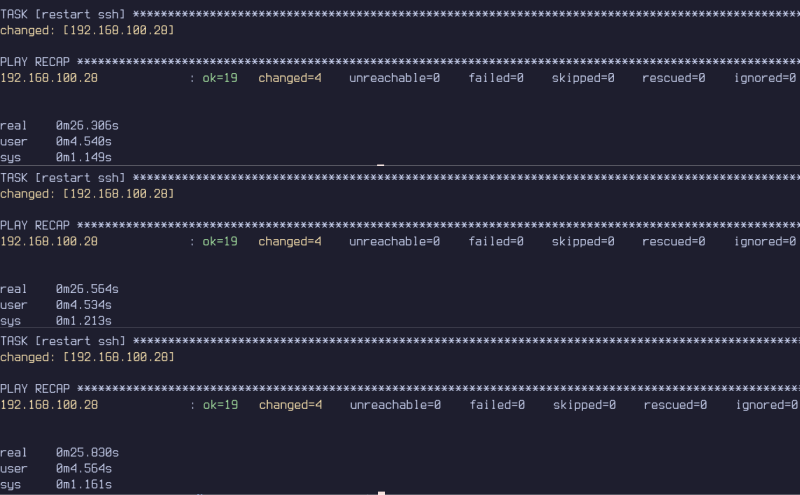
\includegraphics[width=0.8\textwidth]{images/ansible/single/ansible-go-28-com.png}
		\end{center}
		\caption{Ansible second target install Go}
	\end{figure}

	\begin{table}[H]
		\caption{ansible first target}
		\begin{center}
			\begin{tabular}[c]{|c|c|c|c|}
				\hline
				\multicolumn{1}{|c|}{\textbf{Iterasi ke-}} &
				\multicolumn{1}{c|}{\textbf{real}}         &
				\multicolumn{1}{c|}{\textbf{user}}         &
				\multicolumn{1}{c|}{\textbf{sys}}                                            \\
				\hline
				1                                          & 0m34.498s & 0m4.762s & 0m1.237s \\
				\hline
				2                                          & 0m26.016s & 0m4.552s & 0m1.165s \\
				\hline
				3                                          & 0m26.752s & 0m4.584s & 0m1.180s \\
				\hline
			\end{tabular}
		\end{center}
	\end{table}
	\vspace{-5mm}
	\newpage
	\begin{table}[h]
		\caption{ansible second target}
		\begin{center}
			\begin{tabular}[c]{|c|c|c|c|}
				\hline
				\multicolumn{1}{|c|}{\textbf{Iterasi ke-}} &
				\multicolumn{1}{c|}{\textbf{real}}         &
				\multicolumn{1}{c|}{\textbf{user}}         &
				\multicolumn{1}{c|}{\textbf{sys}}                                            \\
				\hline
				1                                          & 0m26.637s & 0m4.281s & 0m1.120s \\
				\hline
				2                                          & 0m26.256s & 0m4.327s & 0m1.027s \\
				\hline
				3                                          & 0m25.256s & 0m4.310s & 0m1.046s \\
				\hline
			\end{tabular}
		\end{center}
	\end{table}
	\subsubsection{Ansible multi target}
	\begin{adjustwidth}{20pt}{}
		Pada percobaan Ansible \textit{multi target}, sama seperti percobaan Ansible \textit{single target}
		pada bagian konfigurasi dan \textit{snapshot}. Namun yang membedakan adalah, perintah
		ansible-playbook dijalankan pada dua target secara paralel. Berikut untuk hasilnya:
	\end{adjustwidth}
	\begin{figure}[h]
		\begin{center}
			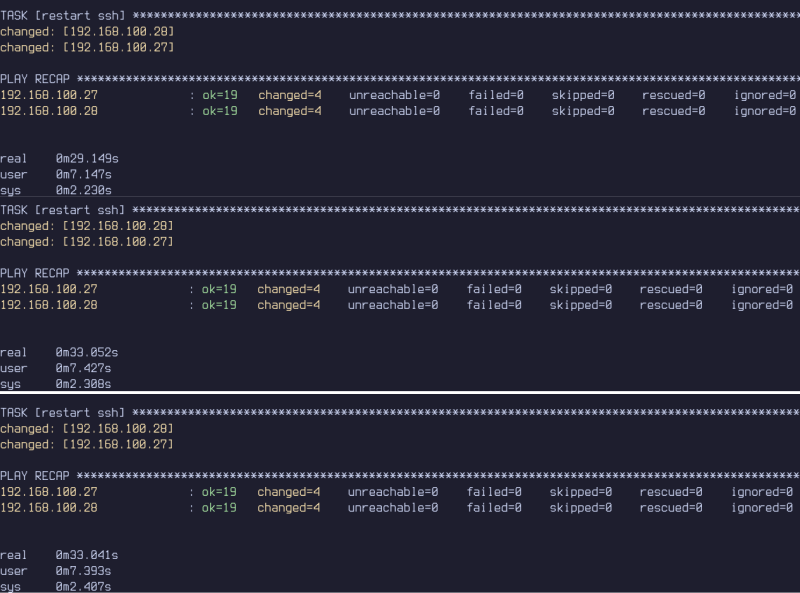
\includegraphics[width=0.9\textwidth]{images/ansible/multi/ansible-go-multi-com.png}
		\end{center}
		\caption{Ansible multi target install Go}
	\end{figure}

	\begin{table}[h]
		\caption{Ansible multi target install Go}
		\begin{center}
			\begin{tabular}[c]{|c|c|c|c|}
				\hline
				\multicolumn{1}{|c|}{\textbf{Iterasi ke-}} &
				\multicolumn{1}{c|}{\textbf{real}}         &
				\multicolumn{1}{c|}{\textbf{user}}         &
				\multicolumn{1}{c|}{\textbf{sys}}                                            \\
				\hline
				1                                          & 0m29.149s & 0m7.147s & 0m2.230s \\
				\hline
				2                                          & 0m33.052s & 0m7.427s & 0m2.308s \\
				\hline
				3                                          & 0m33.041s & 0m7.393s & 0m2.407s \\
				\hline
			\end{tabular}
		\end{center}
	\end{table}
	\subsection{Penghapusan Paket}
	\begin{adjustwidth}{20pt}{}
		Pengujian dilakukan dengan menghapus paket yaitu Go compiler.
		Pengujian ini akan dilakukan tiga kali dengan satu kali perubahan pada file
		konfigurasi.
	\end{adjustwidth}
	\subsubsection{NixOS}
	\begin{adjustwidth}{20pt}{}
		Pada pengujian ini, deskripsi paket Go akan dihapus atau dikomen pada file konfigurasi
		configuration.nix seperti berikut:
		\begin{code}
			\begin{minted}{nix}
        environment.systemPackages = with pkgs; [
          # go
        ];
      \end{minted}
			\caption{Penghapusan paket GO pada konfigurasi NixOS}
		\end{code}
		Perintah nixos-rebuild kemudian dijalankan pada masing-masing target sebanyak tiga
		kali dan hasilnya sebagai berikut:
	\end{adjustwidth}
	\newpage
	\begin{figure}[p]
		\begin{center}
			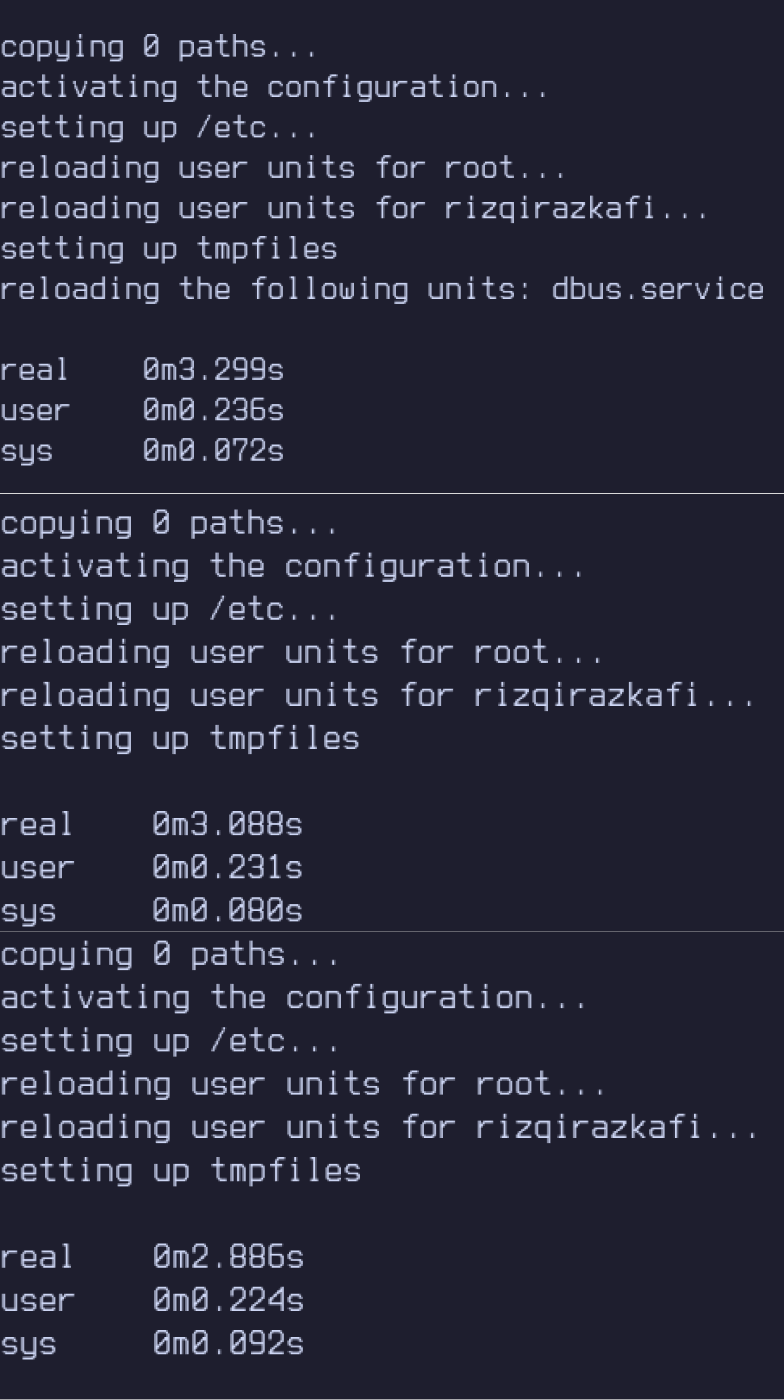
\includegraphics[width=0.8\textwidth]{images/nix-target/nix-remove-go-25-com.png}
		\end{center}
		\caption{nixos-rebuild first target uninstall Go}
	\end{figure}
	\begin{figure}[H]
		\begin{center}
			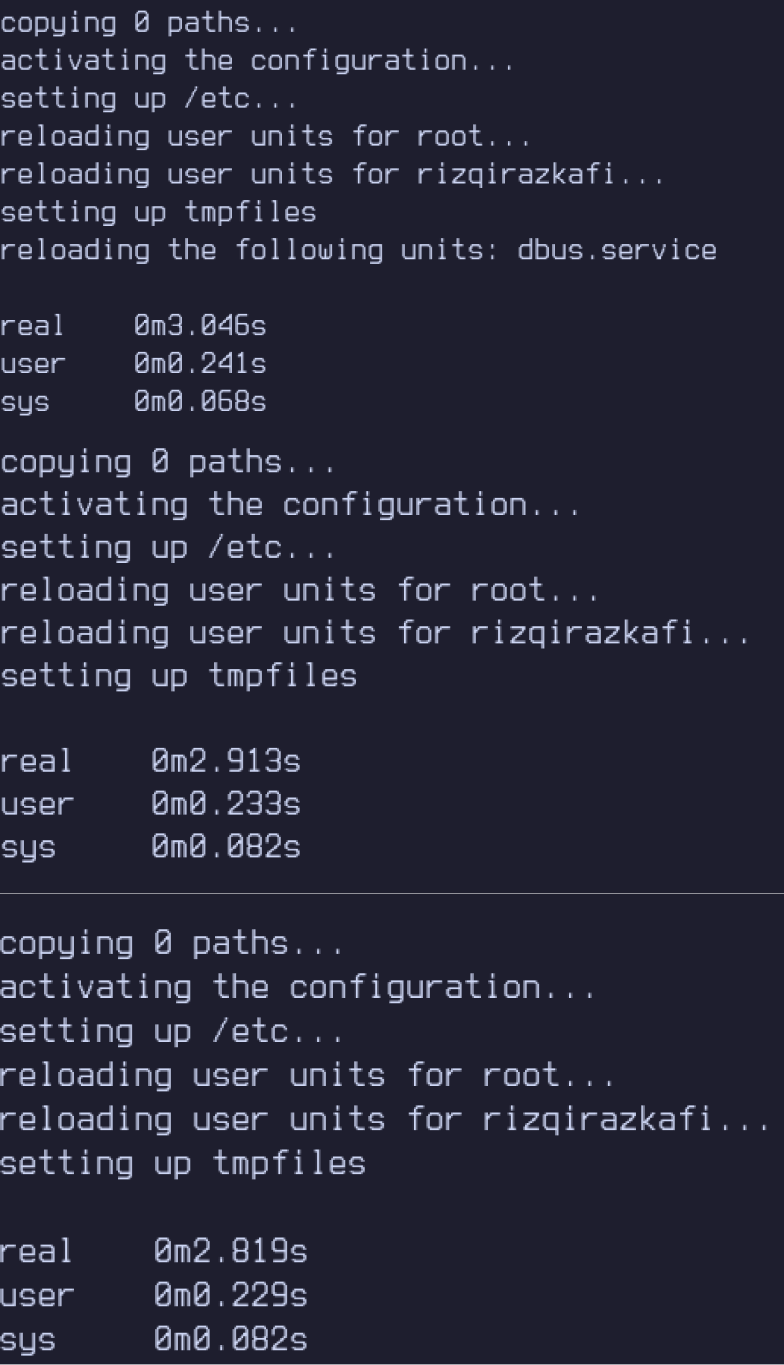
\includegraphics[width=0.8\textwidth]{images/nix-target/nix-remove-go-26-com.png}
		\end{center}
		\caption{nixos-rebuild second target uninstall Go}
	\end{figure}

	\begin{table}[H]
		\caption{nixos-rebuild first target uninstall Go}
		\begin{center}
			\begin{tabular}[c]{|c|c|c|c|}
				\hline
				\multicolumn{1}{|c|}{\textbf{Iterasi ke-}} &
				\multicolumn{1}{c|}{\textbf{real}}         &
				\multicolumn{1}{c|}{\textbf{user}}         &
				\multicolumn{1}{c|}{\textbf{sys}}                                           \\
				\hline
				1                                          & 0m3.299s & 0m0.236s & 0m0.072s \\
				\hline
				2                                          & 0m3.088s & 0m0.231s & 0m0.080s \\
				\hline
				3                                          & 0m2.886s & 0m0.224s & 0m0.092s \\
				\hline
			\end{tabular}
		\end{center}
	\end{table}
	\vspace{-5mm}
	\begin{table}[H]
		\caption{nixos-rebuild second target uninstall Go}
		\begin{center}
			\begin{tabular}[c]{|c|c|c|c|}
				\hline
				\multicolumn{1}{|c|}{\textbf{Iterasi ke-}} &
				\multicolumn{1}{c|}{\textbf{real}}         &
				\multicolumn{1}{c|}{\textbf{user}}         &
				\multicolumn{1}{c|}{\textbf{sys}}                                           \\
				\hline
				1                                          & 0m3.046s & 0m0.241s & 0m0.068s \\
				\hline
				2                                          & 0m2.913s & 0m0.233s & 0m0.082s \\
				\hline
				3                                          & 0m2.819s & 0m0.229s & 0m0.082s \\
				\hline
			\end{tabular}
		\end{center}
	\end{table}
	\subsubsection{Ansible single target}
	\begin{adjustwidth}{20pt}{}
		Untuk Ansible, kita hanya perlu mengganti "\textit{state}" untuk paket Go
		dari "\textit{present}" menjadi "\textit{absent}". Dengan ini kita
		memberitahu Ansible untuk memastikan paket "golang-go" tidak ada pada
		target. Perintah ansible-playbook kemudian dijalankan pada satu target dalam satu
		waktu sebanyak tiga kali dengan hasil dan konfigurasinya adalah sebagai berikut:
		\begin{code}
			\begin{minted}{yaml}
      - name: install go
        ansible.builtin.apt:
          pkg:
            - golang-go
          state: absent
      \end{minted}
			\caption{Konfigurasi penghapusan paket Go pada Ansible}
		\end{code}
	\end{adjustwidth}
	\newpage
	\begin{figure}[H]
		\begin{center}
			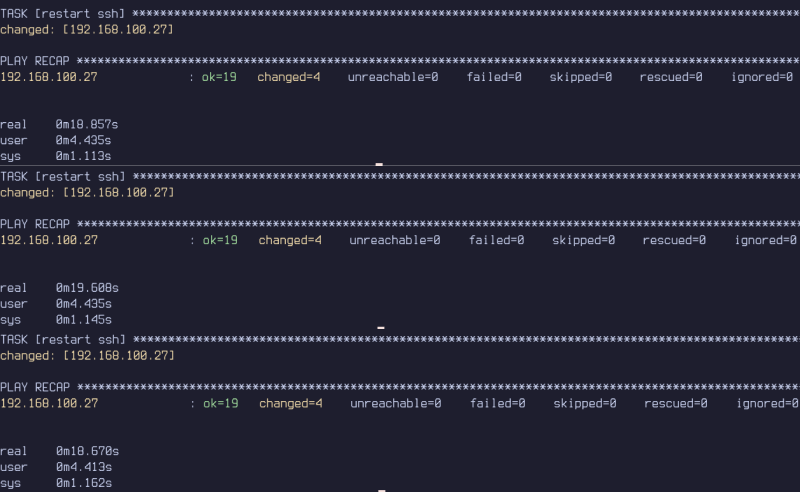
\includegraphics[width=0.95\textwidth]{images/ansible/single/ansible-go-remove-27-com.png}
		\end{center}
		\caption{Ansible first target uninstall Go}
	\end{figure}
	\begin{figure}[H]
		\begin{center}
			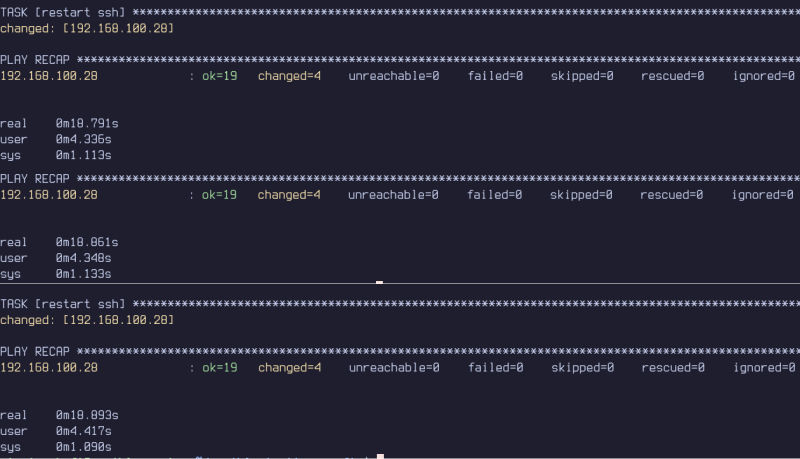
\includegraphics[width=0.95\textwidth]{images/ansible/single/ansible-go-remove-28-com.png}
		\end{center}
		\caption{Ansible second target uninstall Go}
	\end{figure}

	\begin{table}[H]
		\caption{ansible first target}
		\begin{center}
			\begin{tabular}[c]{|c|c|c|c|}
				\hline
				\multicolumn{1}{|c|}{\textbf{Iterasi ke-}} &
				\multicolumn{1}{c|}{\textbf{real}}         &
				\multicolumn{1}{c|}{\textbf{user}}         &
				\multicolumn{1}{c|}{\textbf{sys}}                                            \\
				\hline
				1                                          & 0m18.857s & 0m4.435s & 0m1.113s \\
				\hline
				2                                          & 0m19.608s & 0m4.435s & 0m1.145s \\
				\hline
				3                                          & 0m18.670s & 0m4.413s & 0m1.162s \\
				\hline
			\end{tabular}
		\end{center}
	\end{table}
	\vspace{-5mm}
	\begin{table}[H]
		\caption{ansible second target}
		\begin{center}
			\begin{tabular}[c]{|c|c|c|c|}
				\hline
				\multicolumn{1}{|c|}{\textbf{Iterasi ke-}} &
				\multicolumn{1}{c|}{\textbf{real}}         &
				\multicolumn{1}{c|}{\textbf{user}}         &
				\multicolumn{1}{c|}{\textbf{sys}}                                            \\
				\hline
				1                                          & 0m18.791s & 0m4.336s & 0m1.113s \\
				\hline
				2                                          & 0m18.861s & 0m4.348s & 0m1.133s \\
				\hline
				3                                          & 0m18.893s & 0m4.417s & 0m1.090s \\
				\hline
			\end{tabular}
		\end{center}
	\end{table}
	\subsubsection{Ansible multi target}
	\begin{adjustwidth}{20pt}{}
		Untuk percobaan Ansible \textit{multi target} sama seperti Ansible \textit{single target}.
		Pembedanya terletak hanya di jumlah target yang dituju dimana untuk Ansible \textit{multi target}
		adalah sebanyak dua target dalam percobaan ini. Berikut adalah hasil dari percobaan
		ini:
	\end{adjustwidth}
	\newpage
	\begin{figure}[H]
		\begin{center}
			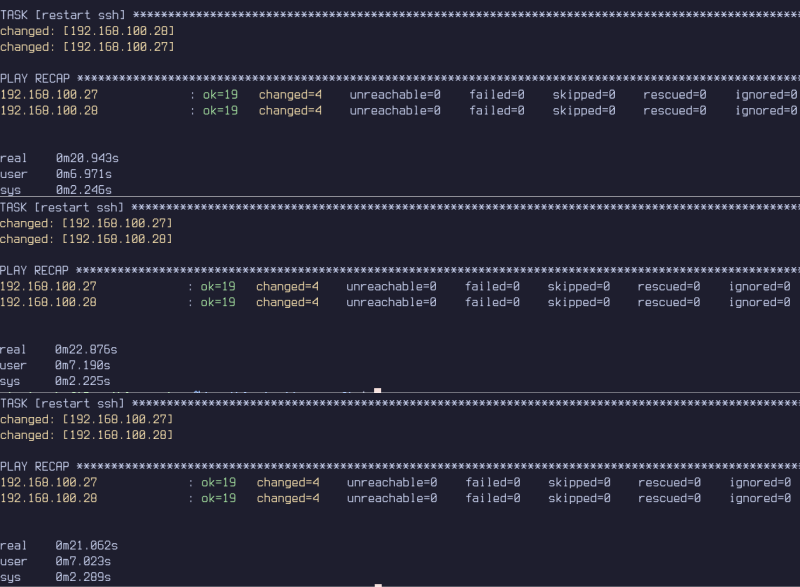
\includegraphics[width=0.95\textwidth]{images/ansible/multi/ansible-go-remove-multi-com.png}
		\end{center}
		\caption{Ansible multi target uninstall Go}
	\end{figure}
	\begin{table}[H]
		\caption{ansible multi target}
		\begin{center}
			\begin{tabular}[c]{|c|c|c|c|}
				\hline
				\multicolumn{1}{|c|}{\textbf{Iterasi ke-}} &
				\multicolumn{1}{c|}{\textbf{real}}         &
				\multicolumn{1}{c|}{\textbf{user}}         &
				\multicolumn{1}{c|}{\textbf{sys}}                                            \\
				\hline
				1                                          & 0m20.943s & 0m6.971s & 0m2.246s \\
				\hline
				2                                          & 0m22.876s & 0m7.190s & 0m2.225s \\
				\hline
				3                                          & 0m21.062s & 0m7.023s & 0m2.289s \\
				\hline
			\end{tabular}
		\end{center}
	\end{table}
	\subsection{Grafik Perbandingan Waktu}
	\begin{adjustwidth}{20pt}{}
		Dari data-data \textit{real time} diatas, maka didapatkan
		rata-rata data grafik waktu yang didapat dalam satuan
		detik adalah sebagai berikut:
	\end{adjustwidth}
	\subsubsection{Pasca Install}
	\begin{adjustwidth}{20pt}{}
		Dalam perhitungan ini, nixos cache, nixos tanpa cache, dan ansible single
		dihitung berdasarkan rata-rata dari 6 kali pengujian dari 2 target yang berbeda.
		Untuk ansible multi, diambil rata-rata dari 3 kali pengujian.
	\end{adjustwidth}
	\begin{tikzpicture}
		\begin{axis}[
				ybar,
				enlargelimits=0.1,
				legend style={at={(0.5,-0.2)},
						anchor=north,legend columns=-1},
				ylabel={waktu dalam detik},
				symbolic x coords={NixOS cache,NixOS tanpa cache,Ansible single,%
						Ansible multi},
				xtick=data,
				nodes near coords,
				nodes near coords align={vertical},
				x tick label style={rotate=45,anchor=east},
			]
			\addplot  coordinates {(NixOS cache,71) (NixOS tanpa cache,209)
					(Ansible single, 130) (Ansible multi, 205)};
		\end{axis}
	\end{tikzpicture}
	\begin{adjustwidth}{20pt}{}
		Dapat kita lihat bahwa NixOS tanpa cache butuh waktu lebih lama dikarenakan
		sistem \textit{package manager} yang akan mengunduh \textit{dependency} tiap
		paket secara terpisah apabila ada perbedaan versi. Faktor lain adalah
		tidak adanya sistem mirror seperti yang dimiliki oleh
		repository Ubuntu dimana paket bisa di simpan di server lain yang dekat, setidaknya
		tidak secara langsung.
		Namun apabila NixOS sudah menyimpan cache, maka NixOS hanya perlu menyalin
		data tersebut ke target dimana kecepatannya bergantung pada koneksi antara
		\textit{host} dan target.

		Untuk Ansible terutama untuk multi target memang rata-rata waktu lebih lama.
		Namun melihat hasil yang didapat dari tiga kali percobaan, waktunya sangat
		fluktuatif dan tidak konsisten.
		Namun apabila kita tambahkan hasil dari NixOS tanpa cache dengan NixOS
		dengan cache, maka total dari rata-ratanya adalah 280 detik untuk
		sekali \textit{build} dan dua kali \textit{copy}.
		Waktu eksekusi untuk NixOS tentu akan bertambah seiring bertambahnya
		target yang perlu di konfigurasi pada satu waktu. Berbeda dengan Ansible yang
		dapat bekerja secara paralel.

	\end{adjustwidth}
	\subsubsection{Penerapan ulang setelah pasca install}
	\begin{tikzpicture}
		\begin{axis}[
				ybar,
				enlargelimits=0.1,
				legend style={at={(0.5,-0.2)},
						anchor=north,legend columns=-1},
				ylabel={waktu dalam detik},
				symbolic x coords={nixos, ansible-single, ansible-multi},
				xtick=data,
				nodes near coords,
				nodes near coords align={vertical},
				x tick label style={rotate=45,anchor=east},
			]
			\addplot coordinates {(nixos, 4.7)
					(ansible-single, 15.83) (ansible-multi, 17.34 )};
		\end{axis}
	\end{tikzpicture}
	\begin{adjustwidth}{20pt}{}
		Disini dapat dilihat Ansible membutuhkan waktu lebih lama untuk melakukan
		pengecekan dikarenakan Ansible melakukan pengecekan tiap \textit{task}
		pada setiap target sedangkan NixOS hanya mengecek perubahan pada konfigurasi
		dan membandingkan \textit{closure} yang ada pada target dengan \textit{host}.
	\end{adjustwidth}
	\subsubsection{Penambahan paket GO}
	\begin{tikzpicture}
		\begin{axis}[
				ybar,
				enlargelimits=0.1,
				legend style={at={(0.5,-0.2)},
						anchor=north,legend columns=-1},
				ylabel={waktu dalam detik},
				symbolic x coords={nixos cache, nixos tanpa cache, ansible single, ansible multi},
				xtick=data,
				nodes near coords,
				nodes near coords align={vertical},
				x tick label style={rotate=45,anchor=east},
			]
			\addplot coordinates {(nixos cache, 13.72)(nixos tanpa cache, 39.32)
					(ansible single, 27.82) (ansible multi, 31.74 ) };
		\end{axis}
	\end{tikzpicture}
	\begin{adjustwidth}{20pt}{}
		Pada grafik diatas, dapat dilihat lagi-lagi NixOS dengan cache lebih unggul
		untuk kasus penambahan paket GO untuk satu target.
	\end{adjustwidth}
	\newpage
	\subsubsection{Penghapusan paket GO}
	\begin{tikzpicture}
		\begin{axis}[
				ybar,
				enlargelimits=0.1,
				legend style={at={(0.5,-0.2)},
						anchor=north,legend columns=-1},
				ylabel={waktu dalam detik},
				symbolic x coords={NixOS, Ansible single, Ansible multi},
				xtick=data,
				nodes near coords,
				nodes near coords align={vertical},
				x tick label style={rotate=45,anchor=east},
			]
			\addplot coordinates {(NixOS, 3)
					(Ansible single, 18.9) (Ansible multi, 21.06)};
		\end{axis}
	\end{tikzpicture}
	\begin{adjustwidth}{20pt}{}
		Pada grafik diatas dapat terlihat bahwa untuk menghapus paket, NixOS
		lebih cepat daripada Ansible. Ini disebabkan karena NixOS tidak langsung menghapus
		paket dari sistem, melainkan hanya mengapus \textit{symlink}. Binary tetap
		disimpan apabila di kemudian hari paket dibutuhkan untuk diinstall kembali.
		NixOS hanya menghapus paket apabila \textit{garbage collector} di eksekusi.
	\end{adjustwidth}
	\subsection{Hasil Konfigurasi}
	\subsubsection{NixOS}
	\begin{adjustwidth}{20pt}{}
		Dapat dilihat bahwa NixOS berhasil mengkonfigurasi target dengan paket dan
		konfigurasi \textit{service} seperti Nginx dan SSH.
		\newpage
		\begin{figure}[H]
			\begin{center}
				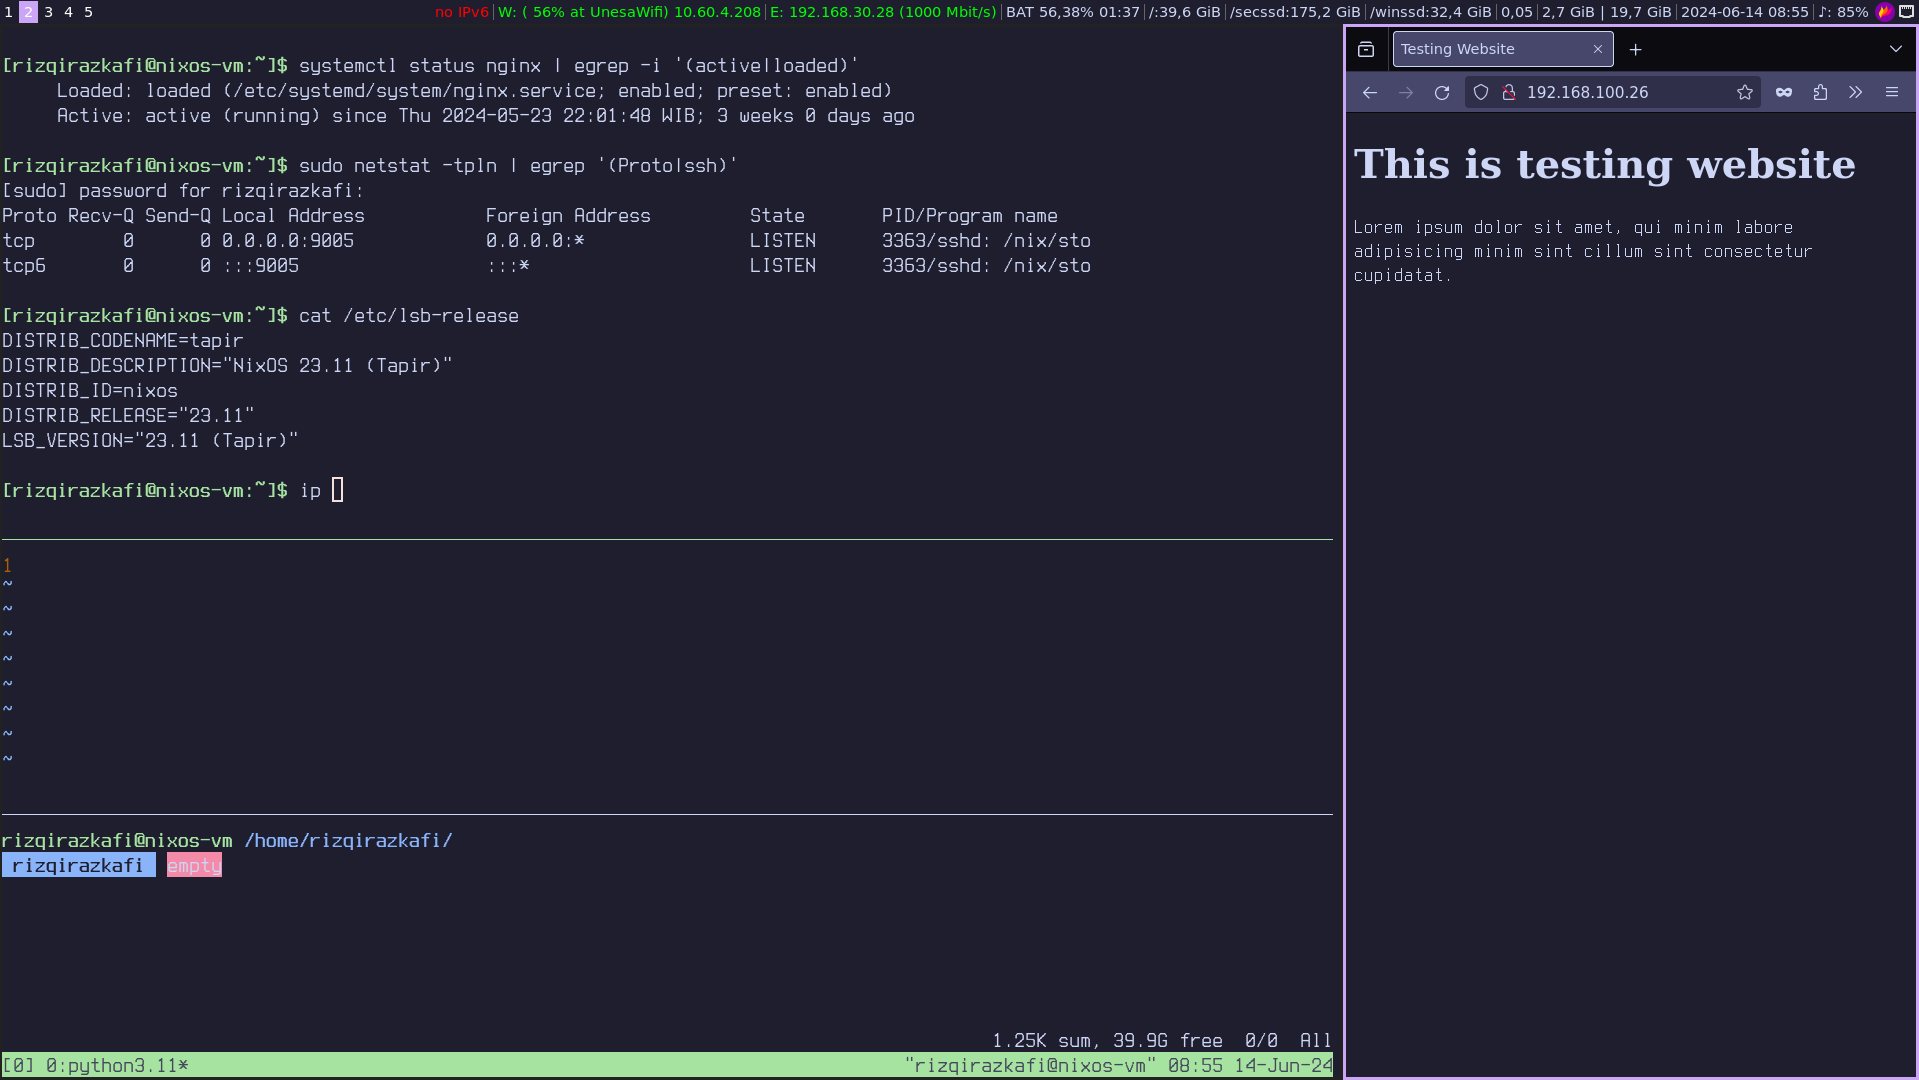
\includegraphics[width=0.95\textwidth]{images/nix-result/result-full-nix.png}
			\end{center}
			\caption{Hasil konfigurasi NixOS}
		\end{figure}
	\end{adjustwidth}
	\subsubsection{Ansible}
	\begin{adjustwidth}{20pt}{}
		Hasil dari Ansible juga menunjukkan bahwa Ansible mampu mengkonfigurasi
		Ubuntu Server sesuai dengan konfigurasi dari keinginan penulis seperti
		dibawah ini
		\begin{figure}[H]
			\begin{center}
				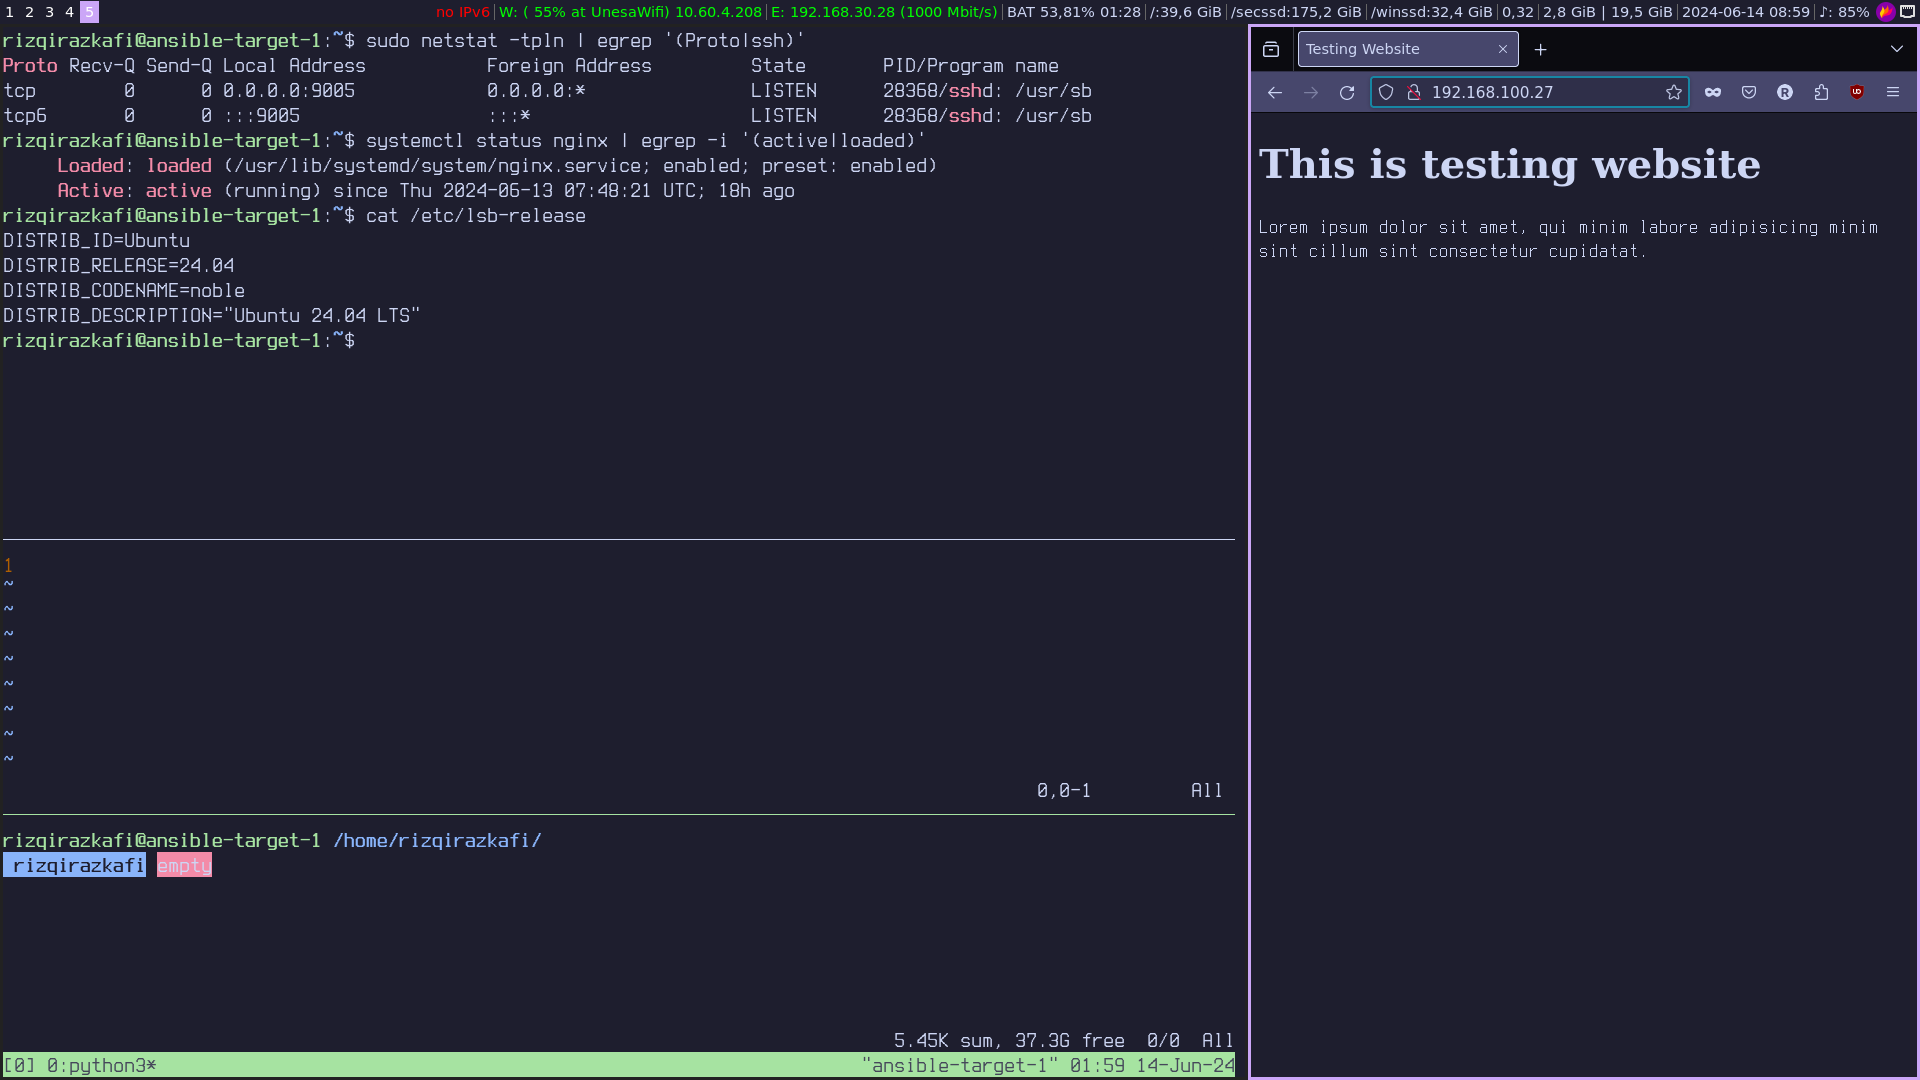
\includegraphics[width=0.95\textwidth]{images/ansible-result/ansible-result-full.png}
			\end{center}
			\caption{Hasil konfigurasi Ansible}
		\end{figure}

	\end{adjustwidth}
	\newpage
	\subsection{Deklaratif dan Imperatif}
	\begin{adjustwidth}{20pt}{}
		Dalam percobaan diatas, terdapat beberapa hal yang ditemui oleh penguji tentang
		\textit{tool} manajemen konfigurasi. Ansible Playbook menggunakan metode imperatif
		dalam praktiknya, dimana Ansible Playbook berisi mengenai apa-apa saja yang harus dilakukan
		oleh Ansible. Ini menyebabkan ketidak cocokan antara Ansible Playbook dengan
		kondisi akhir sistem. Apabila kita mendeskripsikan \textit{task} untuk menginstall
		dan menjalankan Nginx lalu kita terapkan, maka Nginx akan terinstall. Namun
		apabila \textit{task} tersebut dihapus dari Ansible Playbook kemudian kita
		jalankan, maka Nginx akan tetap berjalan.

		Pada sisi lain, konfigurasi NixOS merupakan representasi dari kondisi akhir sistem.
		Apabila kita pada awalnya mendeskripsikan \textit{service} Nginx, maka Nginx akan
		berjalan pada sistem. Apabila kita menghapus pendeskripsian Nginx dari file konfigurasi,
		maka Nginx tidak akan berjalan. Metode inilah yang disebut dengan Deklaratif oleh
		NixOS.

		Sebagai berikut contohnya:
		\begin{code}
			\begin{minted}{nix}
        {
        imports = [
        # Include the results of the hardware scan.
        ./hardware-configuration.nix
        ./vim.nix
        inputs.home-manager.nixosModules.home-manager
        ./nginx.nix
        ];
        }
      \end{minted}
		\end{code}
		Maka Nginx akan di konfigurasi dan berjalan di sistem target seperti berikut:
		\begin{figure}[H]
			\begin{center}
				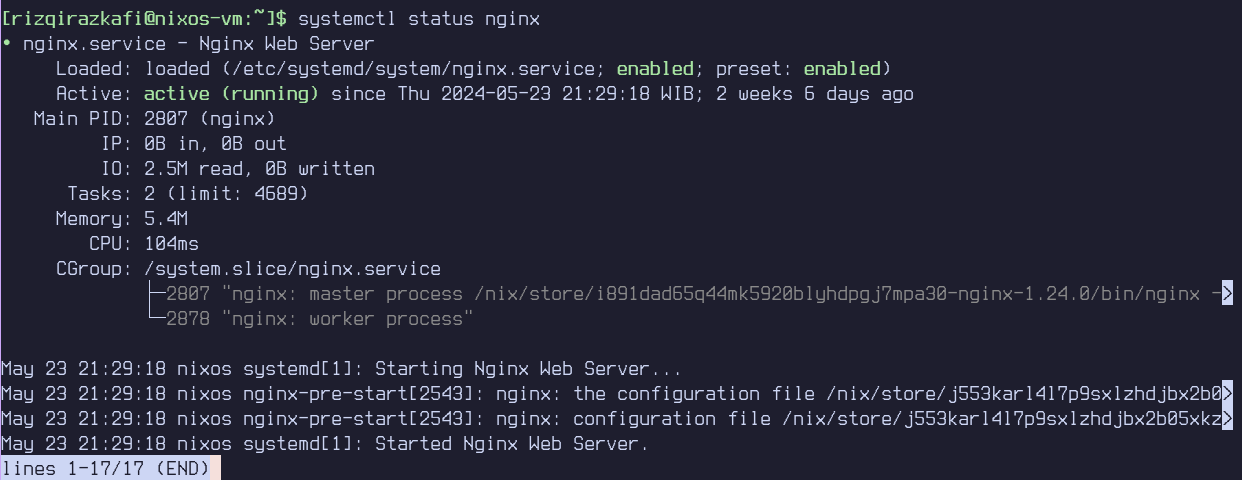
\includegraphics[width=0.8\textwidth]{images/nix-nginx.png}
			\end{center}
			\caption{Nix Nginx enable}
		\end{figure}

		Dan apabila kita ubah sebagai berikut:
		\begin{code}
			\begin{minted}{nix}
        {
        imports = [
        # Include the results of the hardware scan.
        ./hardware-configuration.nix
        ./vim.nix
        inputs.home-manager.nixosModules.home-manager
        # ./nginx.nix
        ];
        }
      \end{minted}
		\end{code}
		Maka hasilnya akan seperti berikut dimana bahkan \textit{service} Nginx
		dihapus dari sistem.
		\begin{figure}[H]
			\begin{center}
				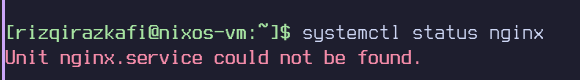
\includegraphics[width=0.8\textwidth]{images/nix-nginx-removed.png}
			\end{center}
			\caption{Nix Nginx removed}
		\end{figure}

		Sedangkan untuk Ansible:
		\begin{code}
			\begin{minted}{yaml}
    tasks:
    - name: install packages
      ansible.builtin.apt:
        pkg:
          - nginx
    tasks: 
    - name: enable nginx
      ansible.builtin.service:
        name: nginx
        state: restarted
      \end{minted}
		\end{code}
		Maka hasilnya akan sebagai berikut:
		\begin{figure}[H]
			\begin{center}
				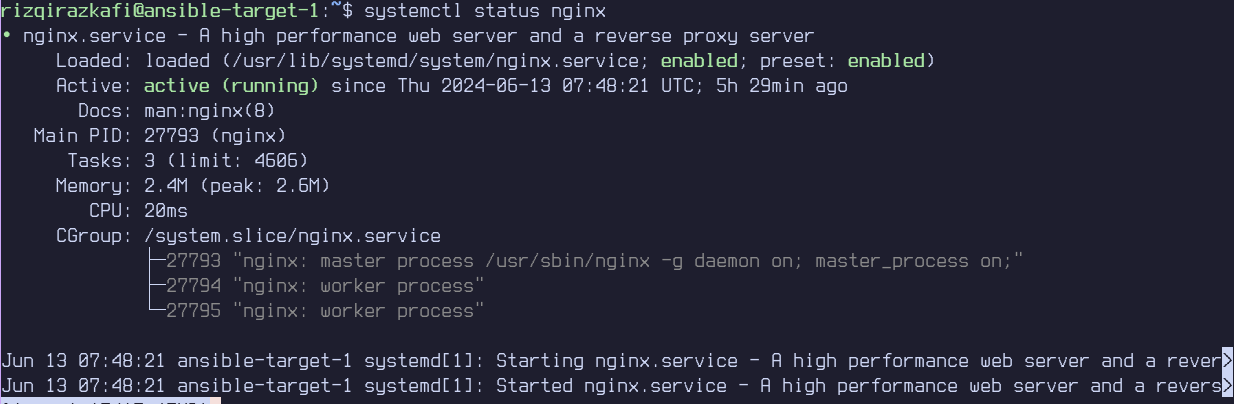
\includegraphics[width=0.8\textwidth]{images/ansible-nginx.png}
			\end{center}
			\caption{Enable nginx}
		\end{figure}
		Dan apabila baris diatas kita beri komentar didepannya, maka hasilnya
		sebagai berikut:
		\begin{figure}[H]
			\begin{center}
				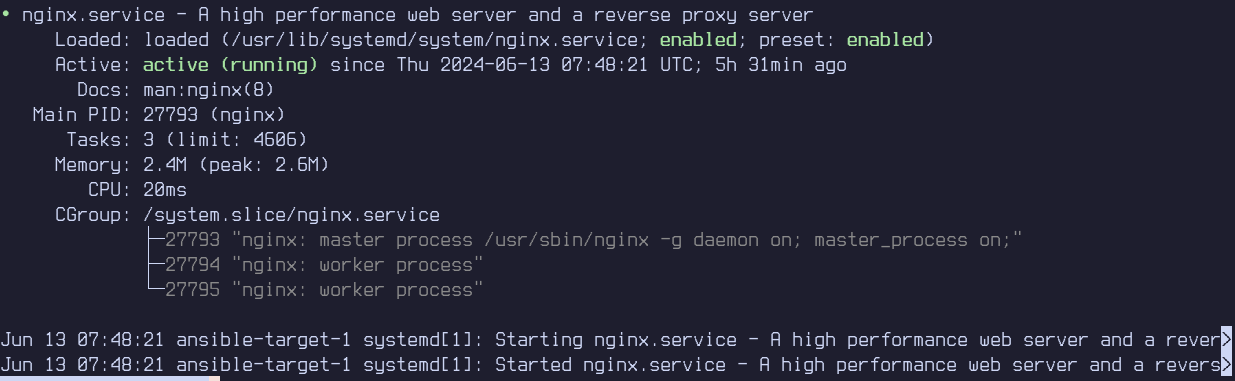
\includegraphics[width=0.95\textwidth]{images/ansible-nginx-2.png}
			\end{center}
			\caption{Nginx masih berjalan}
		\end{figure}
		Hanya jika kita mengganti state dari "enable nginx" ke "stopped" dan mendefinisikan
		"state" dari pkg Nginx ke "absent" barulah Nginx dihentikan dan dihapus dari sistem.
	\end{adjustwidth}
\end{adjustwidth}
% bab V
\chapter{KESIMPULAN DAN SARAN}
\section{Kesimpulan}
\begin{adjustwidth}{20pt}{}
	Berdasarkan penelitian perbandingan performa waktu eksekusi otomasi manajemen
	konfigurasi sistem operasi GNU/Linux antara Ansible dengan NixOS yang telah
	berhasil dilakukan, mendapatkan kesimpulan yang berdasarkan rumusan masalah,
	pembahasan, pengujian, dan hasil penelitian diantaranya:
	\begin{enumerate}[label=\arabic*., nolistsep]
		\item Tujuan penulis adalah membuat sistem manajemen konfigurasi yang
		      deklaratif dimana konfigurasi keseluruhan dari suatu sistem operasi diatur
		      dengan \textit{tool} manajemen konfigurasi. Dari penelitian ini, peneliti
		      mendapati berbagai poin berikut:
		      \begin{enumerate}[label=\alph*., nolistsep]
			      \item Ansible mampu mengkonfigurasi sistem operasi berbasis
			            GNU/Linux (pada kasus ini Ubuntu Server), namun hanya mampu pada
			            tingkat imperatif dan bukan deklaratif.
			      \item NixOS dengan nixos-rebuild mampu mengkonfigurasi sistem
			            operasi berbasis GNU/Linux (pada kasus ini NixOS) secara
			            deklaratif.
		      \end{enumerate}
		\item Setelah melakukan pengujian dari waktu eksekusi kedua \textit{tool}
		      manajemen konfigurasi yaitu Ansible dan NixOS, hasilnya adalah sebagai berikut:
		      \begin{enumerate}[label=\alph*. , nolistsep]
			      \item Dalam uji coba pasca install, urutan waktu eksekusi dari yang tercepat
			            hingga terlambat adalah NixOS dengan cache, Ansible \textit{multi} target,
			            Ansible single target, NixOS tanpa cache.
			      \item Perintah nixos-rebuild tidak dapat digunakan untuk melakukan manajemen
			            konfigurasi secara paralel sedangkan Ansible Playbook dapat dijalankan secara
			            paralel. Ini berdampak pada penerapan dunia nyata dimana semakin banyak
			            target maka waktu yang dibutuhkan untuk penerapan menggunakan nixos-rebuild
			            akan memakan waktu lebih lama walaupun \textit{cache / closure} telah di
			            \textit{build}.
		      \end{enumerate}
	\end{enumerate}
\end{adjustwidth}
\section{Saran}
\begin{adjustwidth}{20pt}{}
	Adapun saran yang dapat diberikan terkait hasil penelitian adalah sebagai berikut:
	\begin{enumerate}[nolistsep]
		\item Disarankan membuat penelitian tentang perbandingan performa waktu eksekusi,
		      maka bisa menggunakan Colmena atau NixOps agar bisa menerapakan konfigurasi NixOS
		      secara paralel.
		\item Disarankan bagi peneliti untuk mengubah jenis penyimpanan target dari HDD
		      ke SSD untuk melihat apakah kecepatan penyimpanan target berpengaruh pada waktu
		      eksekusi.
	\end{enumerate}
\end{adjustwidth}
\addcontentsline{toc}{chapter}{\textbf{DAFTAR PUSTAKA}}
\printbibliography[title={DAFTAR PUSTAKA}]
\end{document}
